\documentclass[xcolor={dvipsnames}]{beamer}
\usepackage{amsmath}
% \usepackage{beamerthemesplit} // Activate for custom appearance
\usepackage{hyperref}
\usepackage{ragged2e}
\usepackage{amssymb}
\usepackage{verbatim}
\usepackage{lmodern}

%\input xy 
%\xyoption{all}
\usepackage[color,matrix,arrow]{xy}
%\usepackage[normalem]{ulem}
%\usepackage{soul}
\usepackage{cancel}
 \usepackage{array}


\title{Probability}
\author{Schwartz}
\date{\today}


\font\domino=domino
\def\die#1{{\domino#1}}

\begin{document}


\frame{\titlepage}
% proposed fixes
% distinguish Unions from joints
% give them proportions of importance for each thing


\frame
{
 \frametitle{Statistics, Data Science, and other Languages}

We need to get stuff ordered differently... there's not time to do it all...
we need to decide what we should actually see -- what is the *most* important?
and put it in that order.  for next time...

\tiny
\begin{columns}
\begin{column}{0.55\textwidth}
\begin{itemize}
\item \emph{acrolect}: dialect considered better than others
\item \emph{basilect}: dialect considered lower status than others
\item \emph{creole}: mixture of a European language combining  one or more other languages spoken as a first language
\item \emph{diglossia}: which a language exists in a formal or literary form and an informal form with each used situationally
\item \emph{interlanguage}: mixture of two languages used by people learning a new language that uses features of the first language mixed with those of the new language
\item \emph{lexicon}:
the total stock of elements that carry meaning
\item \emph{lingua franca}:
language used to communicate by people with different first languages
\item metalanguage: language for discussing language
\item \emph{pidgin}: language of two or more languages for communication by people with different first languages
\item \emph{prose}: ordinary written language, as opposed to poetry
\item \emph{register}:  language used in a particular situation or for communicating with a particular group of people
\item \emph{sublanguage}: 
a variety of language with its own terms and expressions used by a particular group or to talk about a particular subject, for example, the language used by doctors to talk to each other about medicine
\item vernacular: language spoken in a particular group/area, when it is different from the formal written language
\end{itemize}
\end{column}
\begin{column}{0.5\textwidth}
\begin{itemize}
\item Machine languages: interpreted by hardware
\item Assembly languages: machine language wrapper
\item System languages: low-level tasks like memory/process management (e.g. C/++, Java)
\item High-level languages:  machine independent*
\item Scripting languages: very high-level, expressive, and powerful (Python, R, JavaScript, Perl)
\item Embedded languages: executes inside text\\ (e.g. server and client side JavaScript) 
\item Compiled languages:  verify, tee up, then run*
\item Interpreted languages:  run as is (e.g., Python, R)
\item Declarative languages: what, not how (e.g., SQL)
\item Imperative languages: execution of serial orders*
\item Functional languages: functions only (e.g., Lisp)
\item Iterative languages: generators (e.g., Python)
\item Object oriented languages: classes*
\item Procedural languages: functions*$^{\text{plus, e.g., SQL}}$
\item Visual languages: non-text based
\item Esoteric languages: not intended to be used
\item[]
\item[*] C/++, Java, Python, R
\end{itemize}
\end{column}
\end{columns}

}


\frame
{
\normalsize
 \frametitle{Objectives}
\begin{itemize}
\item Probability -- ALL of it
\item[] 
\item<2-> Counting
\item<2-> Random Variables
\begin{itemize}
\item<2-> Marginal, Joint, and Conditional distributions
\end{itemize}
\item<2-> Distributions
\begin{itemize}
\item<2-> Representations: pmf/pdf/mgf/characteristic functions
\item<2-> Examples: Bernoulli, Binomial, Geometric, Multinomial, Poisson 
Uniform, Normal, $\chi^2$, Gamma, Exponential, Beta 
\item<2-> Properties: E, Var, Cov, Cor 
\item[] 
\end{itemize}
\item<3-> Exposure and comfort with a wide range of sophisticated statistical distribution theory concepts and notations

\end{itemize}

}


\frame
{
\normalsize
 \frametitle{Why \emph{I} (Scott) think YOU ($<$you$>$) should care}

If you're
\begin{itemize}
\item Pro $\Longrightarrow$ Refresher
\item Intermediate $\Longrightarrow$ Solidify 
\item Noob $\Longrightarrow$ Exposure (and organization for starting points)\\${}$
\end{itemize}


\begin{enumerate}
\item<2-> Stats is MUSHT in the \emph{\underline{data} science} world 
\begin{itemize}
\item street cred that takes you to the next level and looks impressive
\item show's you're not messing around and you mean to business 
\item \textbf{like um EVERY interview process will ask this shit}
\item[]
\end{itemize}
\item<3-> Maths allow you to \underline{truly, madly, deeply}, get methodology
\begin{itemize}
\item know exactly what it is and does inside out -- no more, no less
\item[]
\end{itemize}
\item<4-> \text{the whole inference/prediction methodology cosmology \emph{`thing'}}
\vspace{-1em}
\begin{itemize}
\item it's part of the general theoretical framework/landscape and all
\end{itemize}
\end{enumerate}
}


\frame
{
 \frametitle{Counting}
\footnotesize
$\textbf{a.k.a., \emph{combinatorics} -- the discipline of mathematics dedicated to \emph{counting}}$\\${}$\\${}$\\

\normalsize
\begin{itemize}
\item Permutation: How many ways can you \emph{permute} things\\
\begin{itemize}
\item<2->[] \underline{Order matters}\\
\item[]<2-> E.g., ABC, BAC, CBA, ACB, CAB, BCA \\${}$\\
\item<3-> There are $\frac{n!}{(n-k)!}$ $k$-sized permutations of $n$ things ($k < n$)
\end{itemize}
\item[]
\item Combination: How many ways can you \emph{combine} things
\begin{itemize}
\item<4->[] \underline{Order \emph{doesn't} \emph{matter}}\\
\item<4->[] E.g., AB, AC, BC \\${}$\\
\item<5-> The number of $k$-sized subsets of $m$ things ($k < m$) is
\item[]<5-> $$\left(\begin{array}{c}n\\k\end{array}\right) = \frac{n!}{(n-k)!\textcolor{red}{k!}}$$
\end{itemize}
\end{itemize}
}

\frame
{
 \frametitle{Counting: the cartesian product}

\begin{itemize}
\item If there are $m$ ways event \textcolor{blue}{$A$} can happen
\item And there are $n$ ways event \textcolor{blue}{$B$} can happen... then?
\item<2->[] Then there are $m\times n$ \textcolor{blue}{$\;(A, B)\;$} can happen
\item[]
\item[]<3-> 
\begin{tabular}{|c|c|c|c|c|c|c|c|c|c|c|}
\hline
& $a_1$ & $a_2$ & $a_3$ & $a_4$ & $a_5$ & $a_6$ & $a_7$ & $a_8$ & $a_9$ & $a_{10}$ \\\hline
$b_1$&&&&&&&&&&\\\hline
$b_2$&&&&&&&&&&\\\hline
$b_3$&&&&&&&&&&\\\hline
$b_4$&&&&&&&&&&\\\hline
$b_5$&&&&&&&&&&\\\hline
\end{tabular}

\item[]
\item<4-> \emph{How many ways can \textcolor{blue}{$\;A\cdot B \cdot C\;$} happen?}

\end{itemize}
}


\frame
{
 \frametitle{Problem 1:}
 
\begin{itemize}
\item I left messages for my parents and three siblings to call me.
\item<2->[] What's the probability the first two calls are from my parents?
\item<2->[] \textcolor{gray}{Assuming the order of callbacks is random...}
\item<3->[] 
\item<3->[v1] 
\item<4->[] 
\vspace{-3em}
\footnotesize \begin{align*}
\Pr(1^{st} \text{call from parent}) \times {} & \Pr(2^{nd} \text{call from parent} | 1^{st} \text{call from parent})\\
\frac{2}{5} \times {} & \frac{1}{4} \textcolor{gray}{ = \frac{2}{20} = \frac{1}{10}}
\end{align*}
\item<5->[v2] 
 \footnotesize \hspace{2em} Number of ways to (a) order 2$P$'s and 3$S$'s and (b) get $PPSSS$ 
\vspace{.5em}
\item<6>[] 
\footnotesize $\quad\;\; \text{(a) } 5!$ 
\item<7>[] 
\vspace{-1.25em}
\footnotesize $\quad\;\; \text{(a) } 5! \text{ and (b) } 2\times1\times3\times2\times1 = 2!3!$
\item<8->[] 
\vspace{-1.25em}
\footnotesize $\quad\;\; \text{(a) } 5! \text{ and (b) }  2\times1\times3\times2\times1 = 2!3! \textcolor{gray}{\; \Longrightarrow \Pr(PPSSS) = \frac{2!3!}{5!} = \frac{1}{10}}$
\vspace{1em}
\item<9->[v3] \footnotesize One way to have parents call first: $PPSSS$
\item<10->[] \footnotesize How many ways to choose first two  $XY\underline{\;\;}\;\underline{\;\;}\;\underline{\;\;}\;$?
\item<11->[]
$$ \left(\begin{array}{c} 5 \\ 2\end{array}\right) \textcolor{gray}{\Longrightarrow \Pr(PPSSS) = 1 \bigg/\left(\begin{array}{c} 5 \\ 2\end{array}\right) = \frac{2!3!}{5!} = \frac{1}{10}}$$
\end{itemize}

}


\frame
{
 \frametitle{Problem 2:}

\vspace{-1em}
\begin{itemize}
\item[] There are k=3 instructors and n=5 students %previously 9 
\item<2->[] The instructors partition student support responsibilities 
\item<3->[] [i.e., each instructor only works with ``their students''] 
\item<4-> \textcolor{Maroon}{How many ways are there to divvy up the workloads between the instructors if each instructor has at least one student?}
\vspace{-2.25em}
\item[]<5-> \huge $$\star\star\star\star\star$$ %\star\star\star\star
\vspace{-3em}
\item[]<6->\huge $$\star\star|\star|\star\star$$ %\star\star\star\star
\vspace{-3em}
\item[]<7->\huge $$|\star\star\;|\star\star\;\star$$ %\star\star\star\star
\vspace{-1.5em}
\item[]<8->$$  \left(\begin{array}{c} n+k-1 \\ k-1\end{array}\right) \;\;= \;\; \left(\begin{array}{c} 7 \\ 2\end{array}\right)$$
\end{itemize}

\vspace{-.25em}
\onslide<9>{
\textcolor{gray}{The world-famous ``stars and bars'' solution}\\
\tiny
\textcolor{NavyBlue}{The way you get good at solving these types of problems is by knowing what the solutions are}
}
}


\begin{frame}[fragile]
 \frametitle{Problem 3:}

\scriptsize

\begin{verbatim}
'''
The scenario: Donald Trump becomes president and make the python built-in
              'set' class illegal. What do we do?
'''
\end{verbatim}
\end{frame}

\begin{frame}[fragile]
 \frametitle{Problem 3:}

\begin{columns}
\begin{column}{.55\textwidth}

\vspace{-1.5em}

\begin{itemize}
\item[]
\footnotesize
\begin{align*}
\Pr(Hillary_{Awesome}) = {} & 0.20\\
Pr(Hillary_{Wins} | Hillary_{Awesome}) = {} & 0.98\\
Pr(Hillary_{Wins} | Hillary_{\cancel{Awesome}}) = {} & 0.90\\{}\\
Pr( Hillary_{Awesome} | Hillary_{Wins} ) = {} & ?
\end{align*}

\item[]<3->
\vspace{-1em}
\footnotesize
\begin{align*}
\Pr(Hillary_{Wins} \& Hillary_{Awesome}) = {} & 0.20 \cdot 0.98\\
\Pr(Hillary_{\cancel{Wins}} \& Hillary_{Awesome}) = {} & 0.20 \cdot 0.02\\
\Pr(Hillary_{Wins} \& Hillary_{\cancel{Awesome}}) = {} & 0.80 \cdot 0.90\\
\Pr(Hillary_{\cancel{Wins}} \& Hillary_{\cancel{Awesome}}) = {} & 0.80 \cdot 0.10\\
\end{align*}

\item[]<4->
\vspace{-1em}
\begin{tabular}{m{1.1cm}|m{1.5cm}m{1.5cm}|m{1.5cm}}  %{c|cc|c}
                           & $\underset{Hillary}{Awesome}$ & $\underset{Hillary}{\cancel{Awesome}}$ & $\underset{Probability}{\text{Marginal}}$\\ \hline
$\quad\;\;\underset{Hillary}{Wins}$ &  $\;\;\;$\textcolor{red}{0.196} & $\;\;\;$\textcolor{red}{0.720} & $\;\;\;$\textcolor{red}{0.916} \\
$\quad\;\;\underset{Hillary}{\cancel{Wins}}$ & $\;\;\;$0.004 & $\;\;\;$0.080 & $\;\;\;$0.084 \\\hline
 $\underset{Probability}{\text{Marginal}}$& $\;\;\;$0.200 & $\;\;\;$0.800 & $\;\;\;$1.000
\end{tabular}

\end{itemize}
\end{column}
\begin{column}{.45\textwidth}

\begin{itemize}
\item[]<2->
\vspace{-2em}
\tiny
\xymatrix{
&& 0.196 \\
& \text{Election} \ar[ur]^{\Pr(Wins|Awesome)}_{0.98} \ar[dr]^{0.02}_{\Pr(\cancel{Wins}|Awesome)} &\\
& &  0.004 \\
\text{Hillary} \ar[ddr]_{\Pr(\cancel{Awesome})}^{0.8} \ar[uur]^{\Pr(Awesome)}_{0.2}&\\
 & & 0.72 \\
& \text{Election} \ar[ur]^{\Pr(Wins|\cancel{Awesome})}_{0.9}  \ar[dr]^{0.1}_{\Pr(\cancel{Wins}|\cancel{Awesome})}&\\
&& 0.08 \\
}
\item[]<5->
\large
\vspace{-1em}
$$\color{red}{\frac{0.196}{0.916}}$$

\end{itemize}
\end{column}
\end{columns}

\begin{itemize}
\item[]<4->
$$\Pr( Hillary_{Awesome} | Hillary_{Wins} ) = \frac{\Pr( Hillary_{Awesome} \& Hillary_{Wins}) }{\Pr(Hillary_{Wins})}$$
\end{itemize}

%U \ar@/_/[ddr]_y \ar@/^/[drr]^x
 %  \ar@{.>}[dr]|-{(x,y)}            \\
 % & X \times_Z Y \ar[d]^q \ar[r]_p
 %                & X \ar[d]_f       \\
 % & Y \ar[r]^g   & Z                

\end{frame}


\frame
{
 \frametitle{Problem 3:}

\begin{columns}
\begin{column}{.55\textwidth}

\vspace{-1.5em}

\begin{itemize}
\item[]
\footnotesize
\begin{align*}
\Pr(Trump_{Fantastic}) = {} & 0.20\\
Pr(DS_{Job} | Trump_{Fantastic}) = {} & 0.98\\
Pr(DS_{Job} | Trump_{\cancel{Fantastic}}) = {} & 0.90\\{}\\
Pr(Trump_{Fantastic} | DS_{Job} ) = {} & ?
\end{align*}

\item[]<3->
\vspace{-1em}
\footnotesize
\begin{align*}
\Pr(DS_{Job} \& Trump_{Fantastic}) = {} & 0.20 \cdot 0.98\\
\Pr(DS_{\cancel{Job}} \& Trump_{Fantastic}) = {} & 0.20 \cdot 0.02\\
\Pr(DS_{{Job}} \& Trump_{\cancel{Fantastic}}) = {} & 0.80 \cdot 0.90\\
\Pr(DS_{\cancel{Job}} \& Trump_{\cancel{Fantastic}}) = {} & 0.80 \cdot 0.10\\
\end{align*}

\item[]<4->
\vspace{-1em}
\begin{tabular}{m{1.1cm}|m{1.5cm}m{1.5cm}|m{1.5cm}}  %{c|cc|c}
                           & $\underset{Fantastic}{Trump}$ & $\underset{\cancel{Fantastic}}{Trump}$ & $\underset{\text{Marginal prob}}{DS}$\\ \hline
$\quad\;\;\underset{Job}{DS}$ &  $\;\;\;$\textcolor{red}{0.196} & $\;\;\;$\textcolor{red}{0.720} & $\;\;\;$\textcolor{red}{0.916} \\
$\quad\;\;\underset{\cancel{Job}}{DS}$ & $\;\;\;$0.004 & $\;\;\;$0.080 & $\;\;\;$0.084 \\\hline
 $\underset{\text{Marginal prob}}{Trump}$& $\;\;\;$0.200 & $\;\;\;$0.800 & $\;\;\;$1.000
\end{tabular}

\end{itemize}
\end{column}
\begin{column}{.45\textwidth}

\begin{itemize}
\item[]<2->
\vspace{-2em}
\tiny
\xymatrix{
&& 0.196 \\
& \text{Election} \ar[ur]^{\Pr(Job{Fantastic})}_{0.98} \ar[dr]^{0.02}_{\Pr(\cancel{Job}|{Fantastic})} &\\
& &  0.004 \\
\text{Hillary} \ar[ddr]_{\Pr({\cancel{Fantastic}})}^{0.8} \ar[uur]^{\Pr({Fantastic})}_{0.2}&\\
 & & 0.72 \\
& \text{Election} \ar[ur]^{\Pr(Job|{\cancel{Fantastic}})}_{0.9}  \ar[dr]^{0.1}_{\Pr(\cancel{Job}|{\cancel{Fantastic}})}&\\
&& 0.08 \\
}
\item[]<5->
\large
\vspace{-1em}
$$\color{red}{\frac{0.196}{0.916}}$$

\end{itemize}
\end{column}
\end{columns}

\begin{itemize}
\item[]<4->
$$\Pr( Trump_{Fantastic} | DS_{Job} ) = \frac{\Pr( Trump_{Fantastic} \& DS_{Job}) }{\Pr(DS_{Job})}$$
\end{itemize}

%U \ar@/_/[ddr]_y \ar@/^/[drr]^x
 %  \ar@{.>}[dr]|-{(x,y)}            \\
 % & X \times_Z Y \ar[d]^q \ar[r]_p
 %                & X \ar[d]_f       \\
 % & Y \ar[r]^g   & Z                

}


\frame
{
 \frametitle{Problem 4:}

\LARGE 
\begin{itemize}
\item[] Three types of fair coins are in an urn: HH, HT, and TT \Huge
\item[] \textcolor{NavyBlue}{You pull a coin, flip it,\\ and it comes up H}
\item[] \huge
\item \textcolor{Maroon}{What is the probability it comes up H if you flip it a second time?}
\end{itemize}

}


\frame
{
 \frametitle{Random Variables}

\begin{itemize}
\item Random Variable $X$ can take on values in the \emph{sample space} $\mathcal{S}$
\item<2-> The actualized values $x$ of $X$ are called \emph{outcomes}, and $x \in \mathcal{S}$ 
\item<3-> An event $E$ is a subset of the sample space, i.e., $E \subset \mathcal{S}$
\item[]
\item[]<4-> 

\hspace{3.5em} 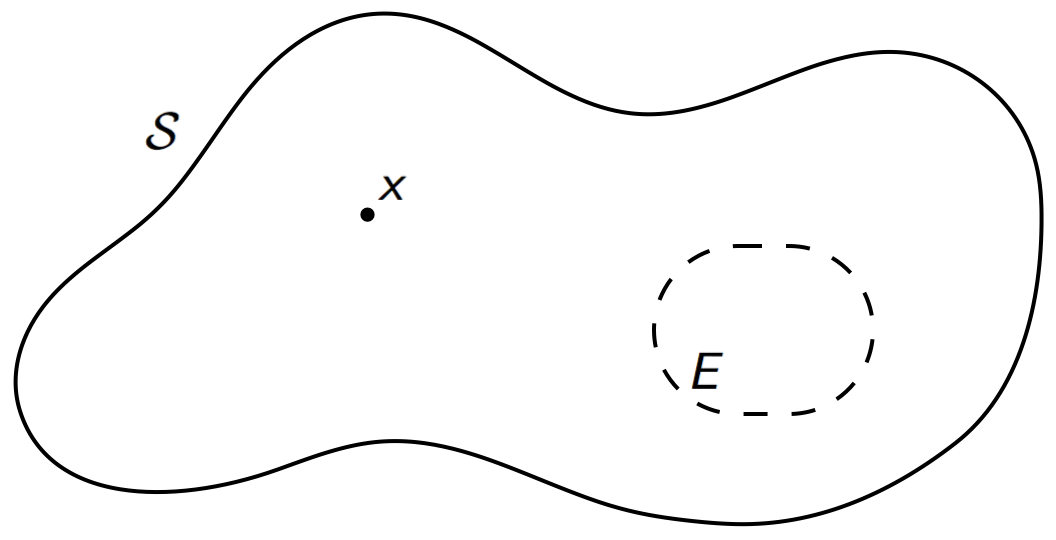
\includegraphics[width=2.5in]{stuff/ss.png}  

\tiny
\hspace{7em}Support space $\mathcal{S}$, event $E$, and outcome $x$ for random variable $X$\\${}$


\item[]<5-> 

\vspace{-10.3em}
\hspace{3.5em} 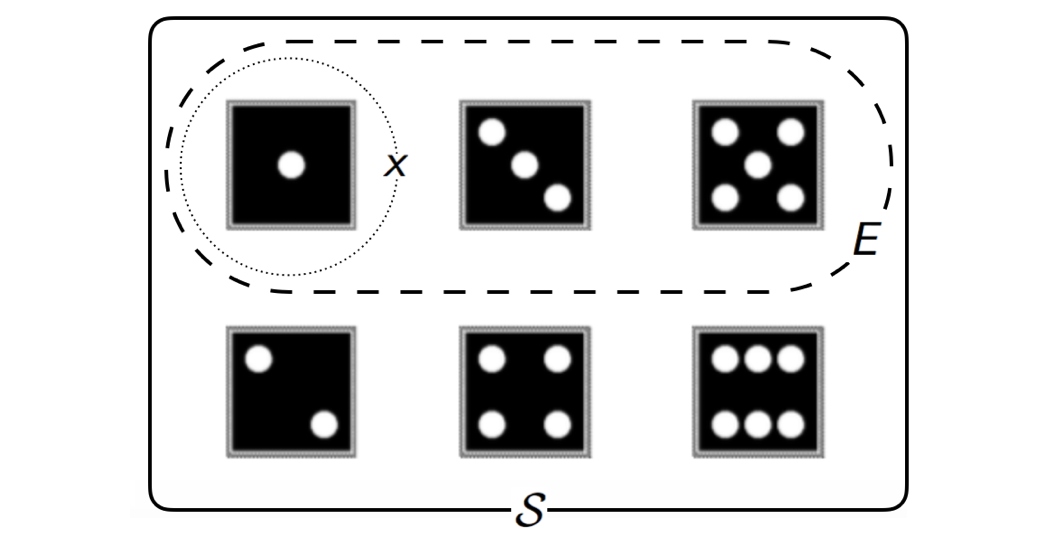
\includegraphics[width=2.5in]{stuff/dice4.png}  

\vspace{2em}

\end{itemize}
}

\frame
{
 \frametitle{Random Variables: Obvious Rules}

\begin{figure}
\centering
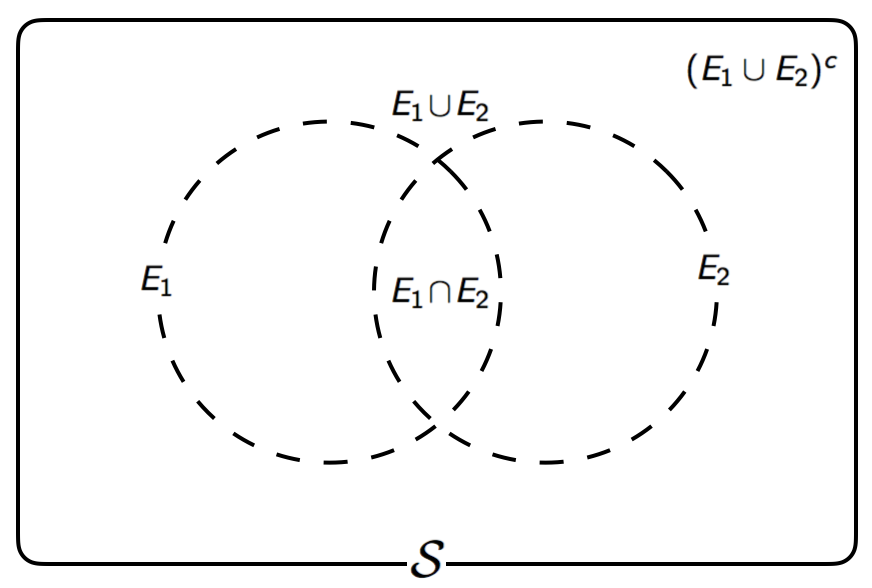
\includegraphics[width=2in]{stuff/venn.png}  \\
Venn Diagram
\end{figure}
\vspace{-1em}
\begin{itemize}
\item $\Pr(E^c) = 1 - \Pr(E)$
\item<2-> $\Pr(E_1 \cup E_2) = \Pr(E_1) + \Pr(E_2) -  \Pr(E_1 \cap E_2)$
\item<3-> $\Pr(E_1 \cap E_2) = \Pr(E_1) + \Pr(E_2) -  \Pr(E_1 \cup E_2)$
\item<4-> $\Pr(E \cap E^c) = 0$
\item<5-> DeMorgan's Laws
\begin{itemize}
\item $\Pr\left((E_1 \cup E_2)^c\right) = Pr\left(E_1^c \cap E_2^c\right) $
\item $\Pr\left((E_1 \cap E_2)^c\right) = Pr\left(E_1^c \cup E_2^c\right)$
\end{itemize}
\end{itemize}
}

\frame
{
 \frametitle{\textcolor{white}{More} Distributions}

%\begin{figure}[h!]
%   \centering
%\hspace*{4cm}
\hspace*{-2.5em}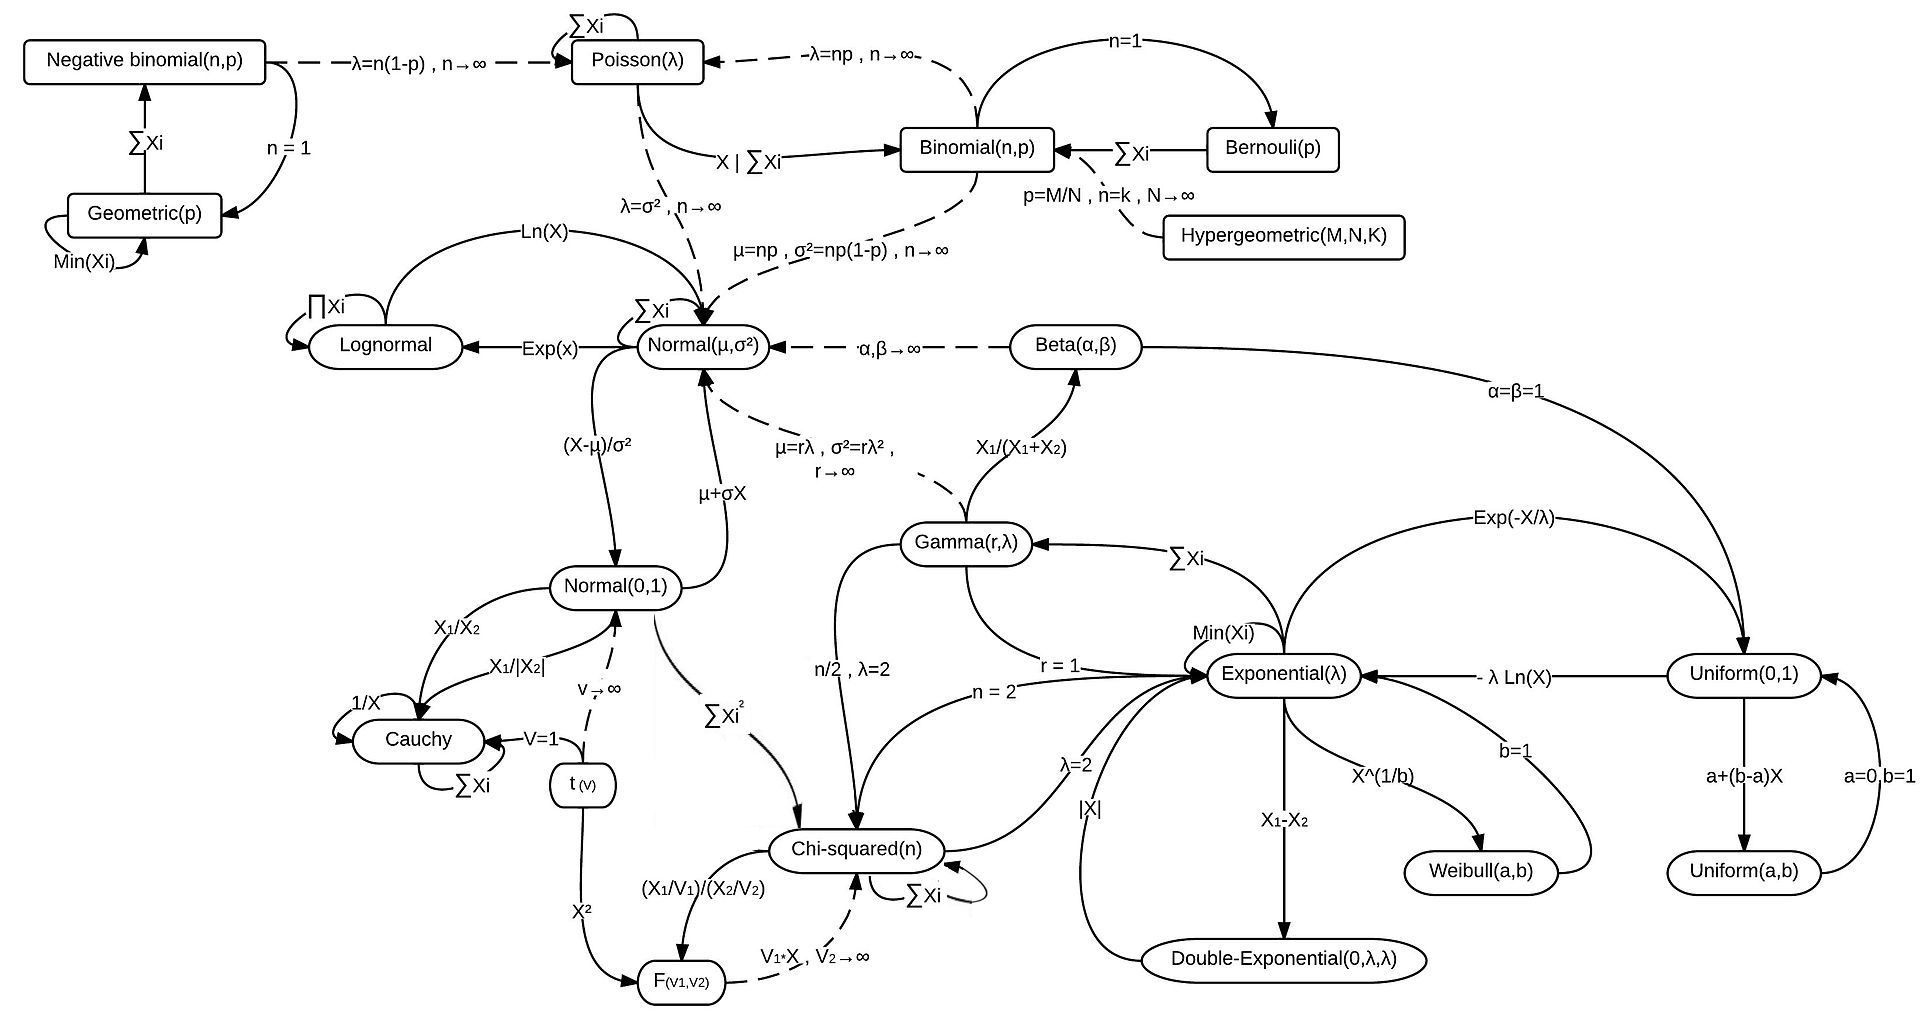
\includegraphics[width=5in]{stuff/relationships.jpg}  
%\end{figure}  
}

\frame
{
 \frametitle{More Distributions}

\vspace{-.5em}
\begin{figure}[h!]
   \centering
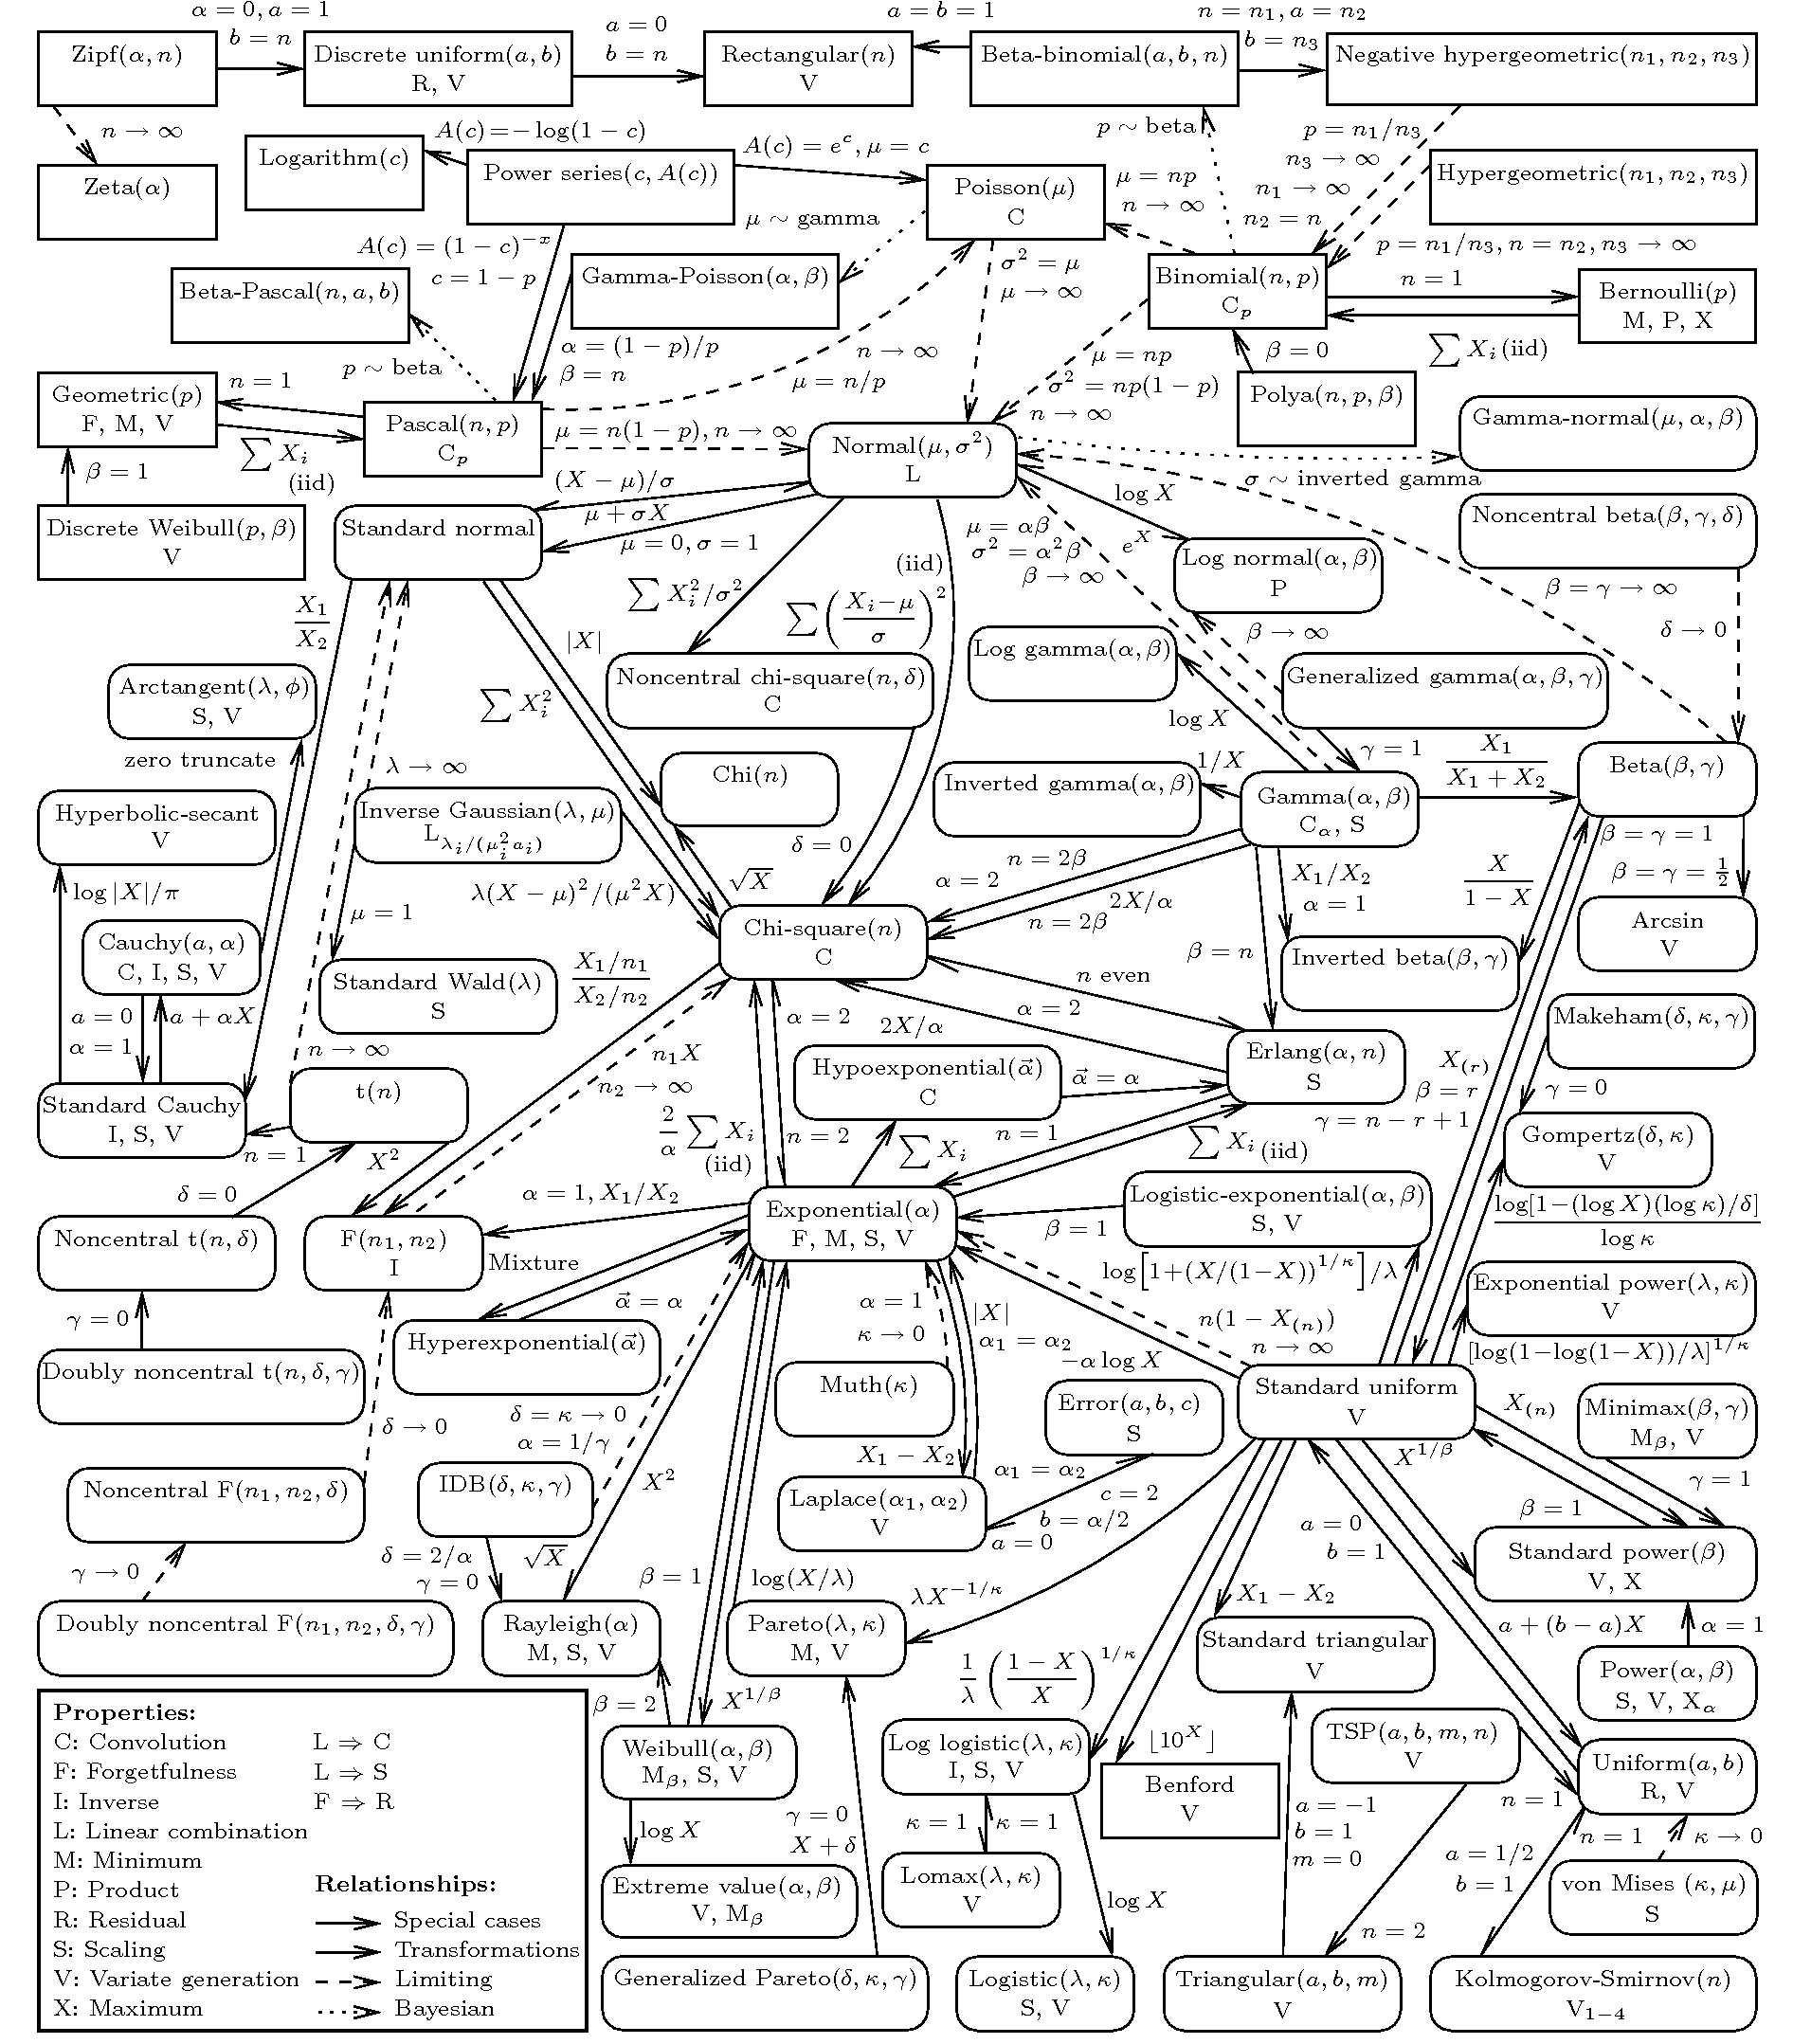
\includegraphics[width=3in]{stuff/connections.png}  
\end{figure}  
}


\frame
{
 \frametitle{Discrete Distributions: \emph{Bernoulli}}
 
 \LARGE
\textcolor{Maroon}{The ``coin flip''}
 
 \huge 
 
\begin{align*}
x \in {} & \left\{0,1\right\} \\\\
\Pr(X=x | p) ={} & p^x(1-p)^{1-x}\\\\
p \in {} & \left[0,1\right]
\end{align*}
}

\frame
{
 \frametitle{Discrete Distributions: \emph{Bernoulli}}

\begin{figure}
\centering
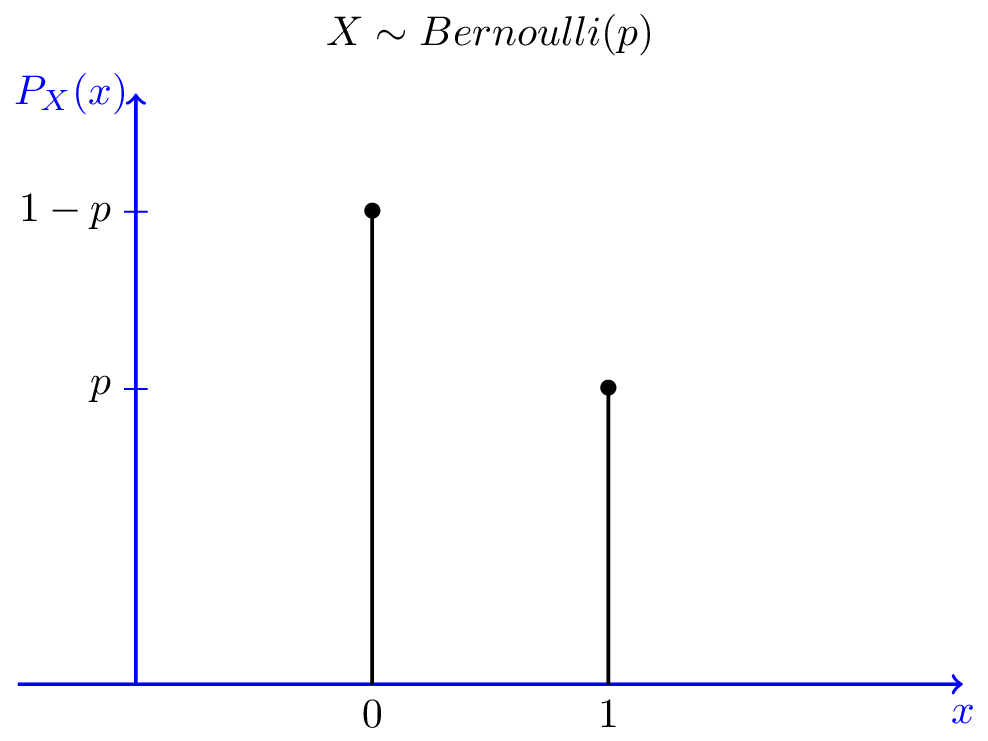
\includegraphics[width=4in]{stuff/bernoulli.png} 
\end{figure}
}

\frame
{
 \frametitle{Discrete Distributions: \emph{Geometric}}

 
 \Large
\textcolor{Maroon}{The ``how many times until''}

 \LARGE
 
\begin{align*}
x \in {} & \left\{0,1,\cdots \infty \right\} \\\\
\Pr(X=x|p) = {} & (1-p)^{x-1}p\\\\
p \in {} & \left[0,1\right]
\end{align*}

\vspace{.25in}
\scriptsize
\emph{"If at first you don't succeed,
Try, try, try again" -- William Edward Hickson}

}

\frame
{
 \frametitle{Discrete Distributions: \emph{Geometric}}

\begin{figure}
\centering
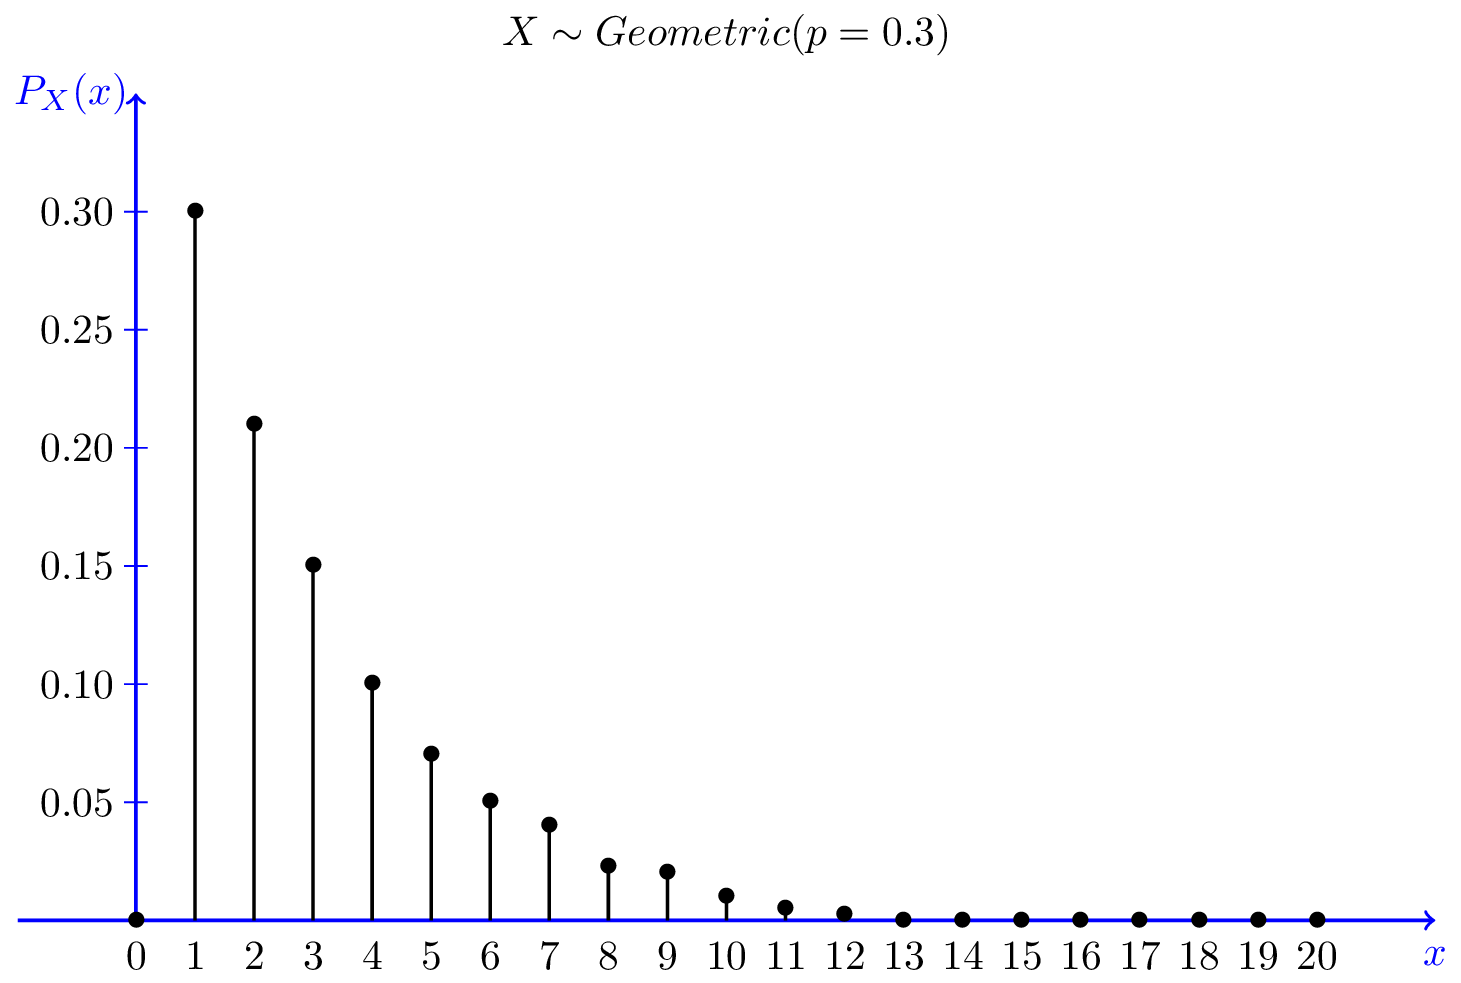
\includegraphics[width=4in]{stuff/geometric.png} 
\end{figure}
}

\frame
{
 \frametitle{Discrete Distributions: \emph{Binomial} }

 \Large
\textcolor{Maroon}{The ``number of success in $n$ trials''}

\LARGE

\begin{align*}
x \in {} & \left\{1,2, \cdots n \right\} \\\\
\Pr(X=x|p,n) = {} & \left(\begin{array}{c}n\\x\end{array} \right)  p^x(1-p)^{n-x}\\\\
p \in {} & \left[0,1\right]
\end{align*}

}

\frame
{
 \frametitle{Discrete Distributions: \emph{Binomial} }
 
\begin{figure}
\centering
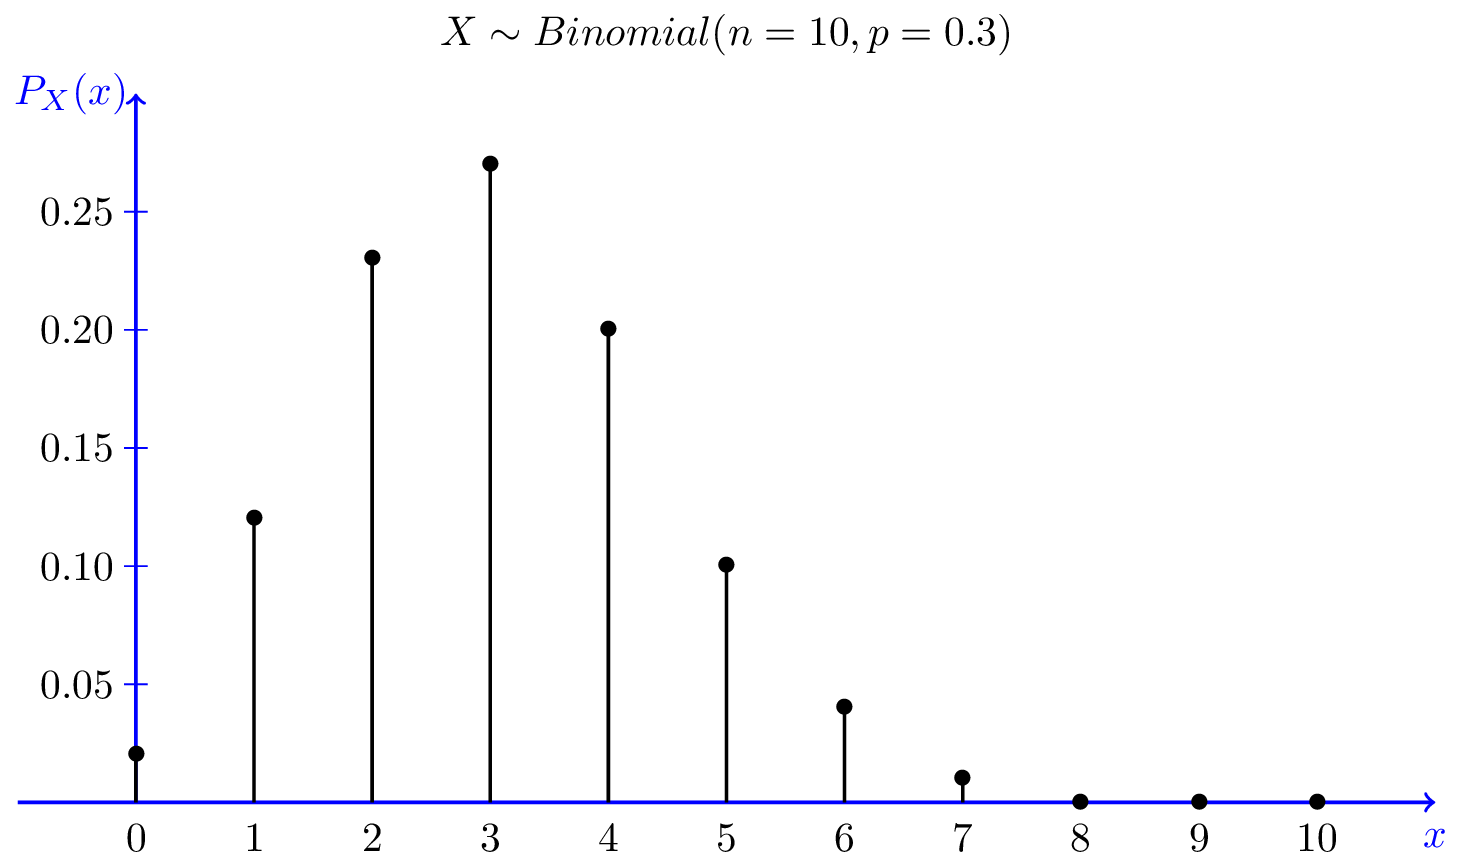
\includegraphics[width=3in]{stuff/binomial1.png}\\${}$

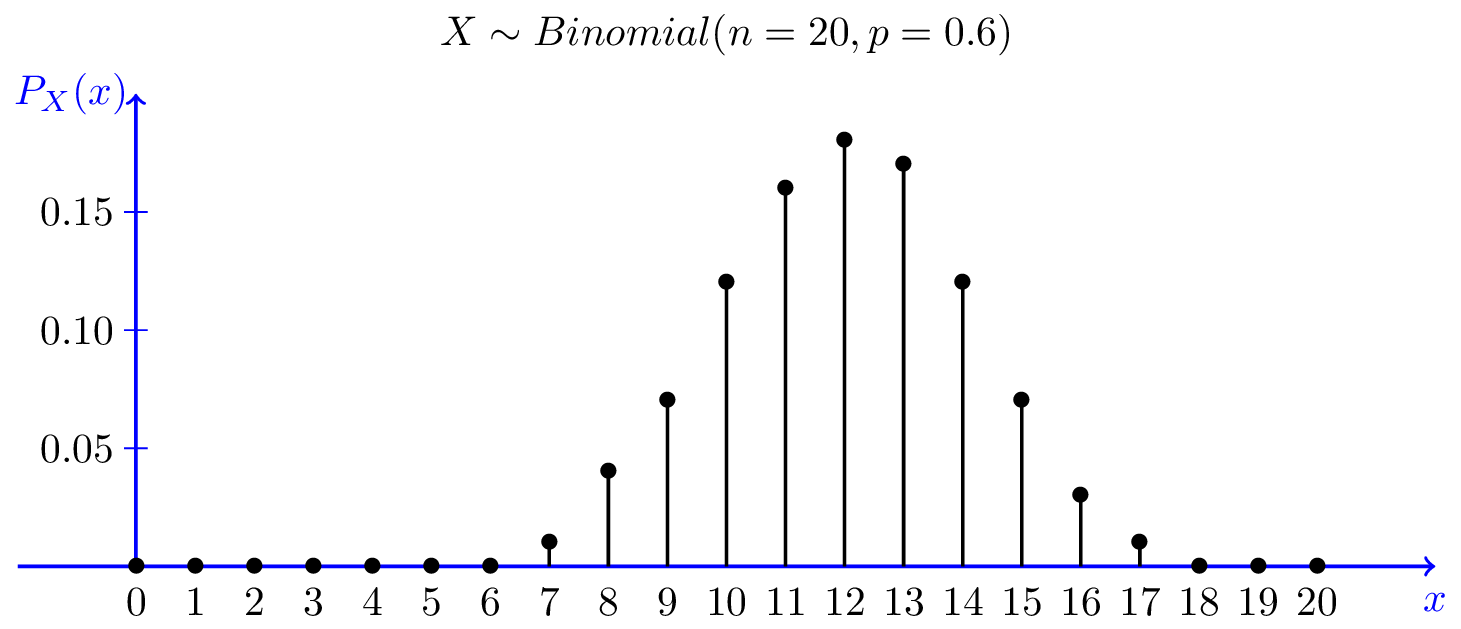
\includegraphics[width=3in]{stuff/binomial2.png} 
\end{figure}
}

\frame
{
 \frametitle{Discrete Distributions: \emph{Multinomial} } 

\Large
 
\textcolor{Maroon}{The ``fancy binomial''}

\large
\begin{align*}
\textbf{x} = {} &(x_1, x_2,\cdots,x_k) \\
x_j \in {} &\left\{0,1, \cdots m \right\}  \text{ such that } \sum x_j  = m 
\end{align*}

\Large

\begin{align*}
\Pr(\textbf{X}=\textbf{x}|\theta_1, \theta_2,\cdots \theta_k, m) 
= {} &\frac{m!}{x_1!x_2!\cdots x_k!}  \prod_{j=1}^k \theta_j^{x_j} \\\\
\theta_j \in {} & \left[0,1\right] \text{ such that } \sum \theta_j  = 1 
\end{align*}


}


\frame
{
 \frametitle{Discrete Distributions: \emph{Poisson}} % binomial approximation/X+Y
 
 \Large

\textcolor{Maroon}{The ``number of arrivals''}

 \LARGE

\begin{align*}
k \in {} & \left\{0,1,\cdots \infty \right\} \\\\
\Pr(X=k|\lambda) = {} &\frac{\lambda^k e^{-\lambda}}{k!}\\\\
\lambda \in {} & \mathbb{R}^+
\end{align*}

}

\frame
{
  \frametitle{Discrete Distributions: \emph{Poisson}} 
  
\begin{tabular}{cc}
  \raisebox{.35em}{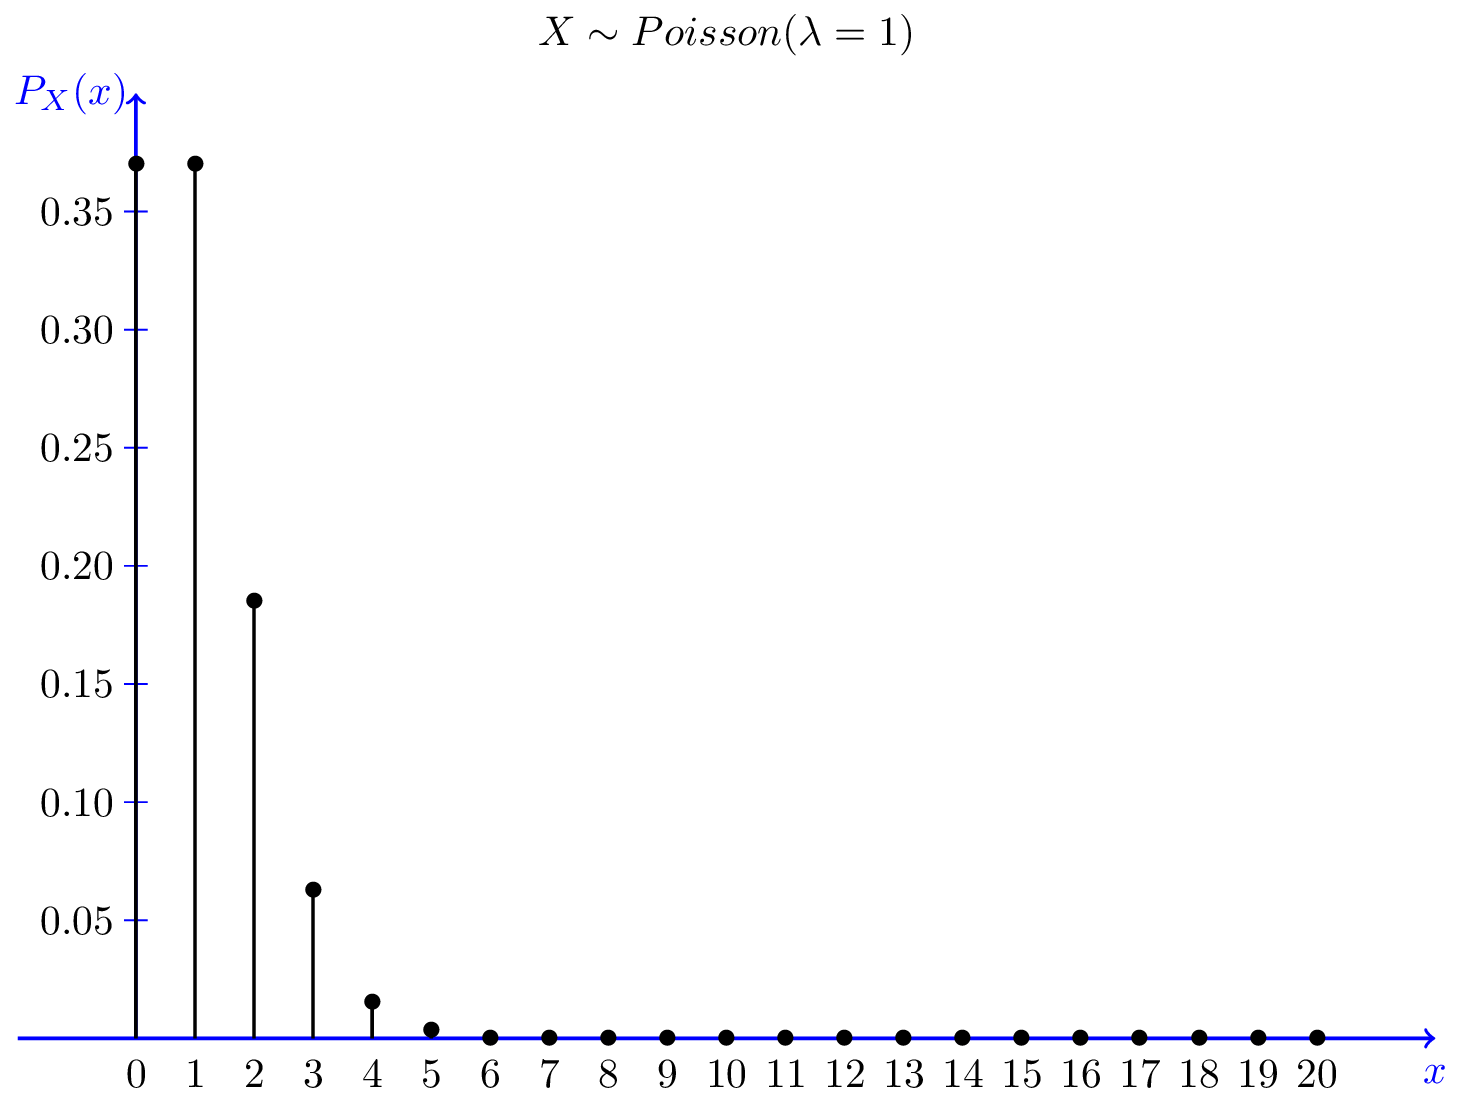
\includegraphics[height=1in]{stuff/Poisson1.png}} & 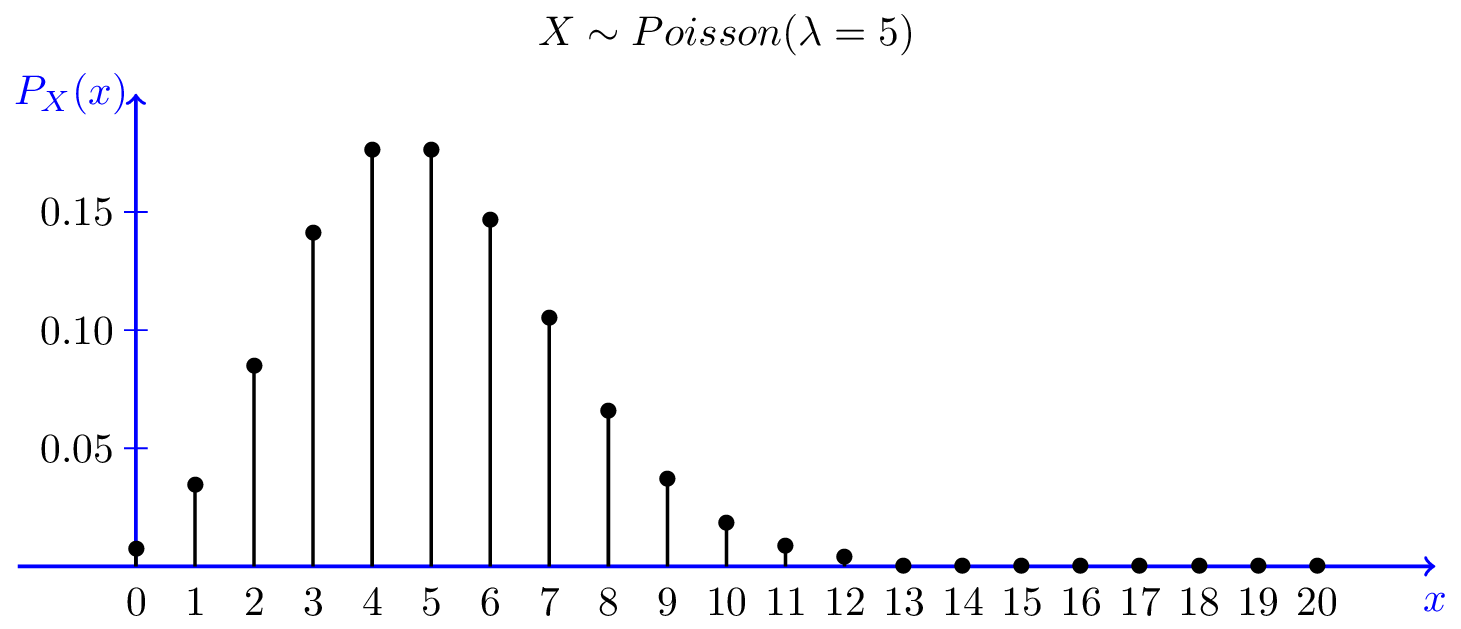
\includegraphics[height=1.1in]{stuff/Poisson2.png}\\
  \end{tabular}

\begin{figure}
\centering
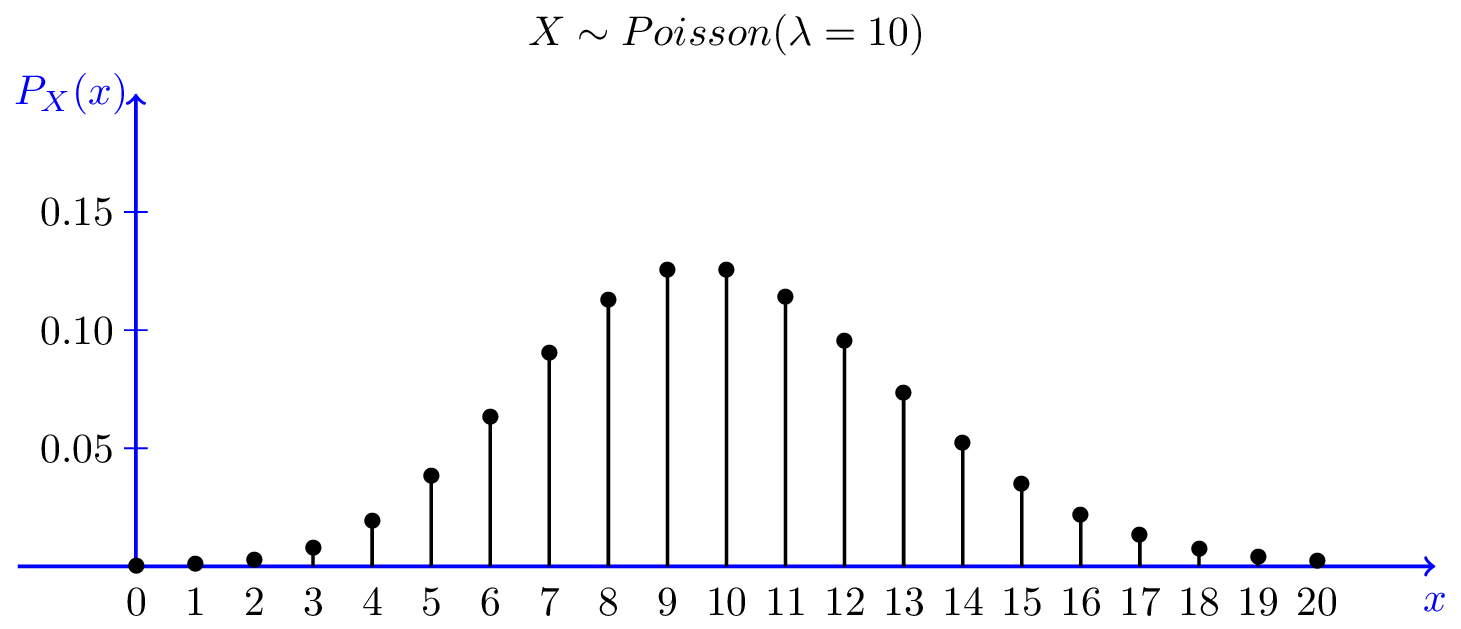
\includegraphics[width=4in]{stuff/Poisson3.png}
\end{figure}
}


\frame
{
 \frametitle{Discrete Distributions: \emph{Poisson} $\approx$ \emph{Bionomial}} % binomial approximation/X+Y

\begin{itemize}
\item If $n \theta = \lambda $ then $\theta  = \frac{\lambda}{n}$ so that

\begin{align*}
 = {} & \left(\begin{array}{c}n\\k\end{array}\right) \theta^k(1-\theta)^{n-k}\\
 = {} & \frac{n\cdot (n-1) \cdots (n - k +1)}{k!} \left(\frac{\lambda}{n}\right)^k\left(1-\frac{\lambda}{n}\right)^{n-k} \\
 = {} & \frac{\textcolor{red}{n\cdot (n-1) \cdots (n - k +1)}}{\textcolor{red}{n^k} k!} \lambda^k\textcolor{blue}{\left(1-\frac{\lambda}{n}\right)^{n}}\textcolor{green}{\left(1-\frac{\lambda}{n}\right)^{-k}} \\
 \approx {} & \frac{\textcolor{red}{1}}{k!} \lambda^k\textcolor{blue}{e^{-\lambda}}\textcolor{green}{1} \;
 \textcolor{gray}{(\text{as } n \rightarrow \infty)} \\
 = {} & \frac{\lambda^k e^{-\lambda}}{k!}
\end{align*}

\end{itemize}

}


\frame
{
 \frametitle{Continuous Distributions: \emph{Uniform}}
 
 \Large

\textcolor{Maroon}{The ``random continuous number''}

\LARGE
 
 \begin{align*}
u \in {} & \mathbb{R} \\\\
f(X=u|a,b) = {} & \frac{1}{b-a} 1_{[a,b]}(u)\\\\
a,b \in {} & \mathbb{R}, a < b
\end{align*}

}



\frame
{
 \frametitle{Discrete Distributions: \emph{Uniform} }
 
\begin{figure}
\centering
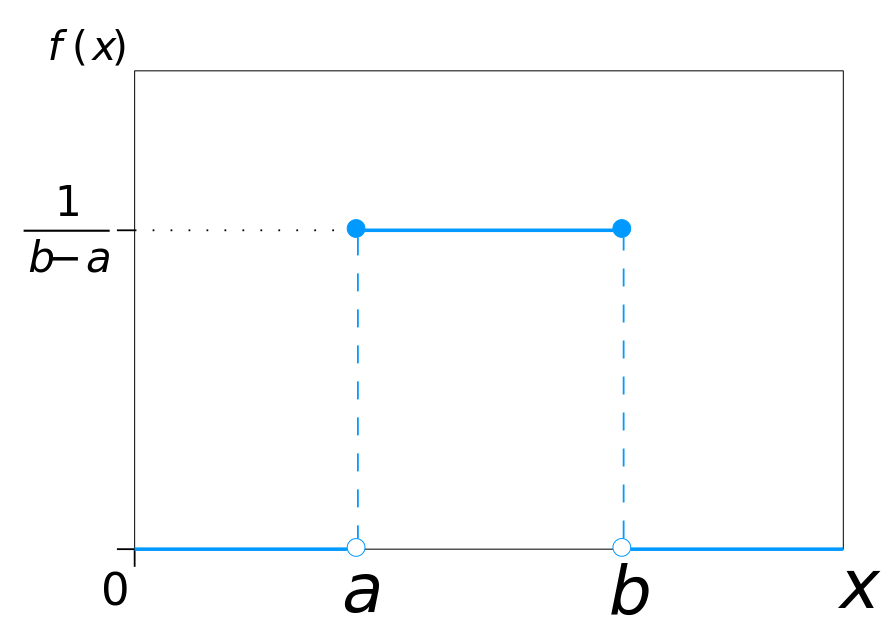
\includegraphics[width=4in]{stuff/uniform.png}
\end{figure}
}



\frame
{
 \frametitle{Continuous Distributions: \emph{Normal}}
 
 \Large

\textcolor{Maroon}{The ``bell curve''}

\LARGE
 
\begin{align*}
x \in {} & \mathbb{R} \\\\
f(X=x|\mu,\sigma^2) = {} & \frac{1}{\sqrt{2\pi \sigma^2}} e^{-\frac{1}{2\sigma^2}(x-\mu)^2}\\\\
\mu \in {} & \mathbb{R}, \sigma^2 \in \mathbb{R}^+
\end{align*}
 
}

\frame
{
 \frametitle{Continuous Distributions: \emph{Normal} }
 
\begin{figure}
\centering
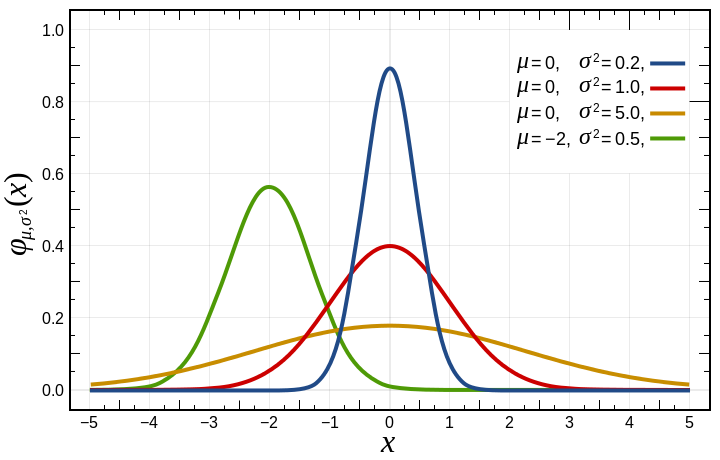
\includegraphics[width=4in]{stuff/normal.png}
\end{figure}
}

\frame
{
 \frametitle{Continuous Distributions: $Normal^2$}
 
\begin{itemize}
\item If $X_j \sim Normal\left(\mu,\sigma^2\right)$ are normal random variables
\item[]<2->
$$Z_j = \frac{X_i-\mu}{\sigma}$$
\item[]<3-> are standard normal random variables 
\item[]<4-> $$\text{i.e., } Z_j \sim Normal\left(0,1\right), \text{ and}$$ 
\item[]<5->
$$ \sum_{j=1}^k Z_i^2 \sim \chi^2_k$$
\item[]<6-> is \emph{chi-squared} random variable with $k$ ``degrees of freedom'' 
\item[]
\item[]<7-> The $\chi^2_{df}$ distribution is a key distribution in hypothesis testing
\end{itemize} 
 }


\frame
{
 \frametitle{Continuous Distributions: $Normal^2: \chi^2_{df}$ }
 
\begin{figure}
\centering
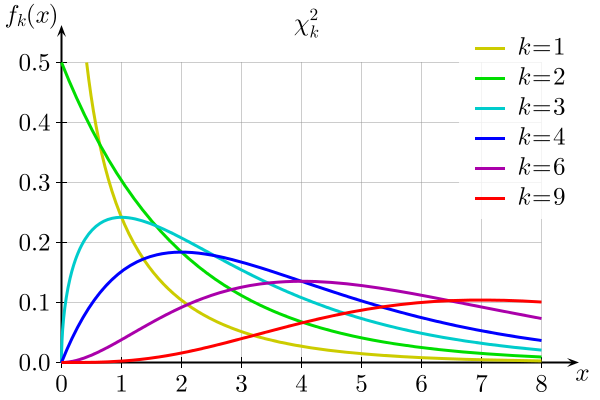
\includegraphics[width=4in]{stuff/chi2.png}
\end{figure}
}




\frame
{
 \frametitle{Continuous Distributions: \emph{Gamma}} %(exponential (aging property), chi-squared
 
 \Large

\textcolor{Maroon}{The ``Bayesian model for variance'' }

\LARGE
 
\begin{align*}
x \in {} & \mathbb{R}^+ \\\\
f(X=x|\theta,k) = {} & \frac{\theta^k}{\Gamma(k)} x^{k-1} e^{-x\theta}\\\\
\theta \in {} & \mathbb{R}^+
\end{align*}
}

\frame
{
 \frametitle{Continuous Distributions: \emph{Gamma}}
 
\begin{figure}
\centering
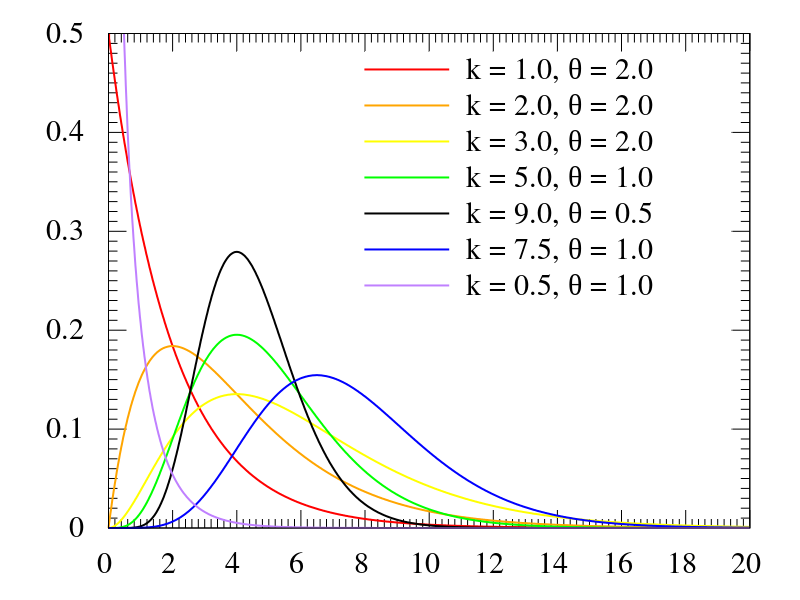
\includegraphics[width=4in]{stuff/gamma.png}
\end{figure}
}



\frame
{
 \frametitle{Continuous Distributions: \emph{Gamma ($\theta = 1/2$, Chi-squared)}} %(exponential (aging property), chi-squared

\begin{itemize}
\item \textcolor{gray}{We previously derived the $\chi^2_{df}$ distribution as the ``sum of squared standard normal distributions''}
\item \textcolor{gray}{and noted its importance in hypothesis testing}  
\item[] \textcolor{Maroon}{The $\chi^2_{df}$ is also a special case of the gamma distribution}

\LARGE

\vspace{-.75em}

\begin{align*}
x \in {} & \mathbb{R}^+ \\
f(X=x|k) = {} & \frac{\frac{1}{2}^{\frac{k}{2}}}{\Gamma\left(\frac{k}{2}\right)} x^{\frac{k}{2}-1} e^{-\frac{x}{2}}\\
k \in {} & \mathbb{R}^+
\end{align*}

\vspace{.25em}

\normalsize
\item[] \textcolor{NavyBlue}{Bonus: if $X\sim\chi^2_{v}$ and $X\sim\chi^2_{w}$, then 
$\frac{\frac{1}{v}\chi^2_{v}}{\frac{1}{w}\chi^2_{w}} \sim F_{v,w}$}
\end{itemize}

}

\frame
{
 \frametitle{Continuous Distributions: \emph{Gamma ($\theta = 1/2, \chi^2_{df}$)}}
 
\begin{figure}
\centering
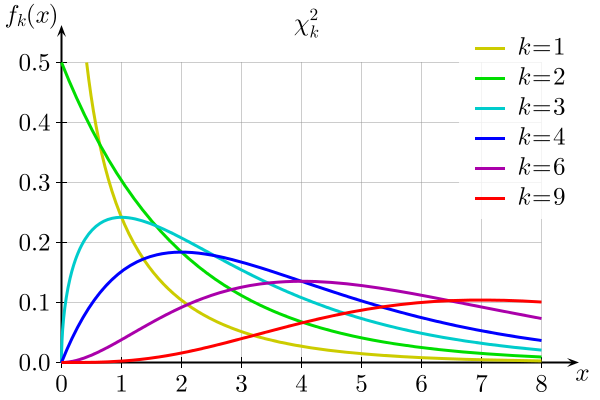
\includegraphics[width=4in]{stuff/chi2.png}
\end{figure}
}


\frame
{
 \frametitle{Continuous Distributions: \emph{Gamma (k=1, Exponential)}} %(exponential (aging property), chi-squared

 \vspace{.5em}
\textcolor{Maroon}{The \emph{Exponential} is another special case of the gamma}

 
 \vspace{-.75em}
\LARGE
 
\begin{align*}
x \in {} & \mathbb{R}^+ \\\\
f\left(X=x|\theta\right) = {} & \theta e^{-x\theta}\\\\
\theta \in {} & \mathbb{R}^+
\end{align*}

 \vspace{.5em}

\normalsize 

\begin{itemize} 
\item \textcolor{NavyBlue}{The Exponential is often used to model time to failure}
\item \textcolor{NavyBlue}{It has an interesting ``ageless'' property, however, in that
$$ \Pr(X=x+c|x=0) = \Pr(X=x+c|x) \text{ for any value of $x$}$$}
\end{itemize}

}

\frame
{
 \frametitle{Continuous Distributions: \emph{Gamma (k=1, Exponential)}}
 
\begin{figure}
\centering
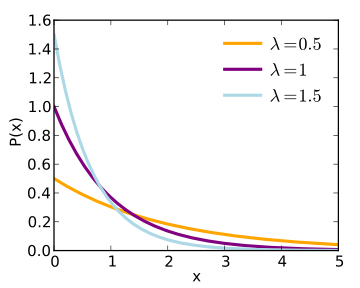
\includegraphics[width=4in]{stuff/exponential.png}
\end{figure}
}

 





\frame
{
 \frametitle{Continuous Distributions: \emph{Beta}}

\large
\textcolor{Maroon}{The ``distribution for modeling random probabilities''}

\vspace{-.75em}
\LARGE

\begin{align*}
p \in {} & [0,1] \\\\
f(X=p|\alpha, \beta) = {} & \frac{\Gamma(\alpha + \beta)}{\Gamma(\alpha)\Gamma(\beta)} p^{\alpha-1} (1-p)^{\beta-1}\\\\
\alpha, \beta \in {} & \mathbb{R}^+
\end{align*}

\vspace{.5em}

\normalsize
\textcolor{NavyBlue}{$\alpha = \beta = 1$ results in a \emph{uniform distribution} over the unit interval}
}

\frame
{
 \frametitle{Continuous Distributions: \emph{Beta}}
 
\begin{figure}
\centering
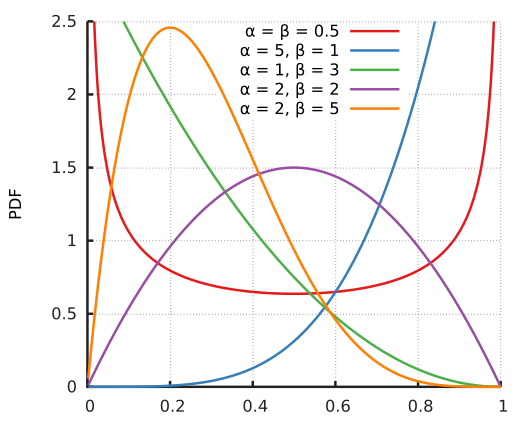
\includegraphics[width=4in]{stuff/beta.png}
\end{figure}
}

 
 
 \frame
{
 \frametitle{$PDF/PMF$, $CDF$, and characteristic functions} % binomial approximation/X+Y

\begin{columns}
\begin{column}{.6\textwidth}

\begin{enumerate}
\item We have thus far defined the distribution of a random variable\\ 
in terms of the \underline{\emph{PDF and PMF}} %$\Pr(X = x|\theta)$
\item[]
\item We can equivalently alternatively define the distribution of $X$ by it's \underline{\emph{cumulative distribution function}} %$\Pr(X \leq x|\theta)$
\item[]
\end{enumerate}
\end{column}
\begin{column}{.4\textwidth}
\begin{figure}
\vspace{-2em}
\hspace{-4.5em}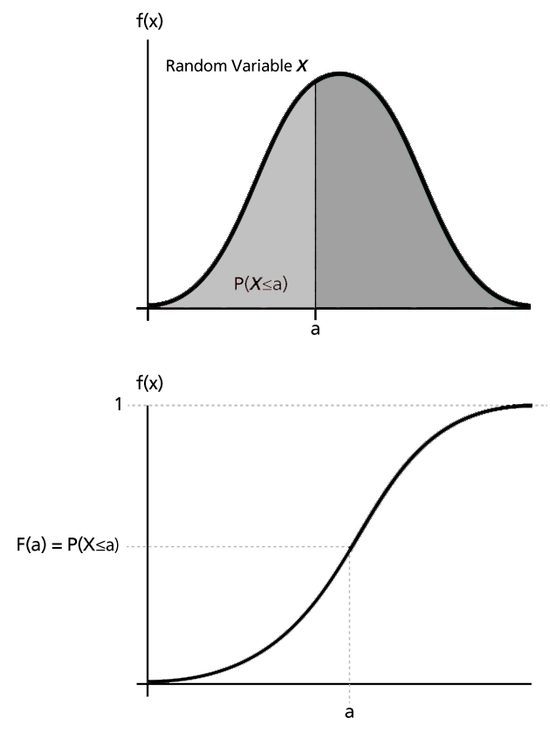
\includegraphics[width=1.25in]{stuff/pdfCDF.png}
\end{figure}
\end{column}
\end{columns}


\begin{itemize}
\item[3.]<2-> \textcolor{NavyBlue}{Yet another way to define the distribution of $X$ is by its 
\emph{moment generating function} or its \emph{characteristic function}: 
$$\text{E}\left[tX\right], \text{ or } \text{E}\left[itX\right], \text{ respectively}$$}
\vspace{-1em}
\item[]<3-> \textcolor{Maroon}{Interestingly, the characteristic function of $X + Y$
for \emph{independent} random variables $X$ and $Y$ is the product \\ of the characteristic functions of $X$ and $Y$}
\end{itemize}
}

\frame
{
 \frametitle{Discrete Distributions: \emph{Poisson} + \emph{Poisson}} % binomial approximation/X+Y

\begin{itemize}
\item The characteristic function of a \emph{Poisson} random variable is 
$$e^{\lambda\left(e^{it}-1\right)}$$
\item<2-> For $X$ and $Y$ Poisson distributed random variables with parameters $\lambda_X$
and $\lambda_Y$, the characteristic function of $X + Y$ is
$$e^{\lambda_X\left(e^{it}-1\right)}e^{\lambda_Y\left(e^{it}-1\right)} = e^{(\lambda_X+\lambda_Y)\left(e^{it}-1\right)}$$
\item[]<3-> So $X + Y$ is Poisson distributed with parameter $\lambda_X+\lambda_Y$
\item[]
\item<4-> Quiz: name the distributions of $X+X$ and $Y+Y$ if 
$$X \sim Bernoulli(\theta) \text{ and } Y \sim Binomial(\theta,n )$$
with respective characteristic functions 
$$1 - \theta + \theta e^{it} \text{ and } \left(1 - \theta + \theta e^{it}\right)^n$$
\end{itemize}

}
 
 
\frame
{
 \frametitle{Continuous Distributions: $Normal + Normal$}
 
\begin{itemize}
\item The characteristic function of a normal random variable is
$$ e^{it\mu -\frac{1}{2}t^2\sigma^2}$$
\item[]<2-> What is the distribution of $X + Y$ if
$$ X \sim Normal\left(\mu_X,\sigma^2_X\right) \text{ and }  Y \sim Normal\left(\mu_Y,\sigma^2_Y\right)?$$
\end{itemize} 
}


\frame
{
 \frametitle{Continuous Distributions: $X_1+X_2+\cdots+X_n \sim Normal $}
 \scriptsize
 
\begin{itemize}
\item The moment generating function (MGF) of a normal random variable is
$$ e^{t\mu + \frac{1}{2}t^2\sigma^2}$$ 
\item[]<2-> The MGF of the sum of $n$ \emph{arbitrary} $i.i.d.$ random variables 
$\sum_{i=1}^n X_i$ is 
$$\left(1 + t \text{E}[X] + \frac{t^2 \text{E}[X^2]}{2!} + \frac{t^3 \text{E}[X^3]}{3!} + \cdots\right)^n$$ 
\item[]<3-> Using $\log\left((1+u)^n\right) = n\left(u - \frac{u^2}{2!} + \frac{u^3}{3!} - \cdots \right)$, we have
\item[]<4->
\begin{align*}
{} & \exp\left(n\left(  t \text{E}[X] + \frac{t^2 \text{E}[X^2]}{2} + \cdots -  \frac{t^2 \text{E}[X]^2}{2} - \cdots + \cdots  \right)\right)\\
 = & e^{t n\text{E}[X] + \frac{1}{2}t^2 n(\text{E}[X^2] - \text{E}[X]^2) + n(\cdots )}\\
\approx {} & e^{t n\text{E}[X] + \frac{1}{2}t^2 n(\text{E}[X^2] - \text{E}[X]^2)} \text{
as $n \rightarrow \infty \;$ \onslide<5->{\textcolor{gray}{so $\sum_{i=1}^n X_i \sim N(n\text{E}[X], n(\text{E}[X^2] - \text{E}[X]^2))$}}} 
\end{align*}
\footnotesize
\onslide<6->{\textcolor{NavyBlue}{The binomial distribution with large $n$ is approximately normal: why?}}
\end{itemize} 
}



\frame
{
 \frametitle{Joint Distributions}

\begin{figure}
\centering
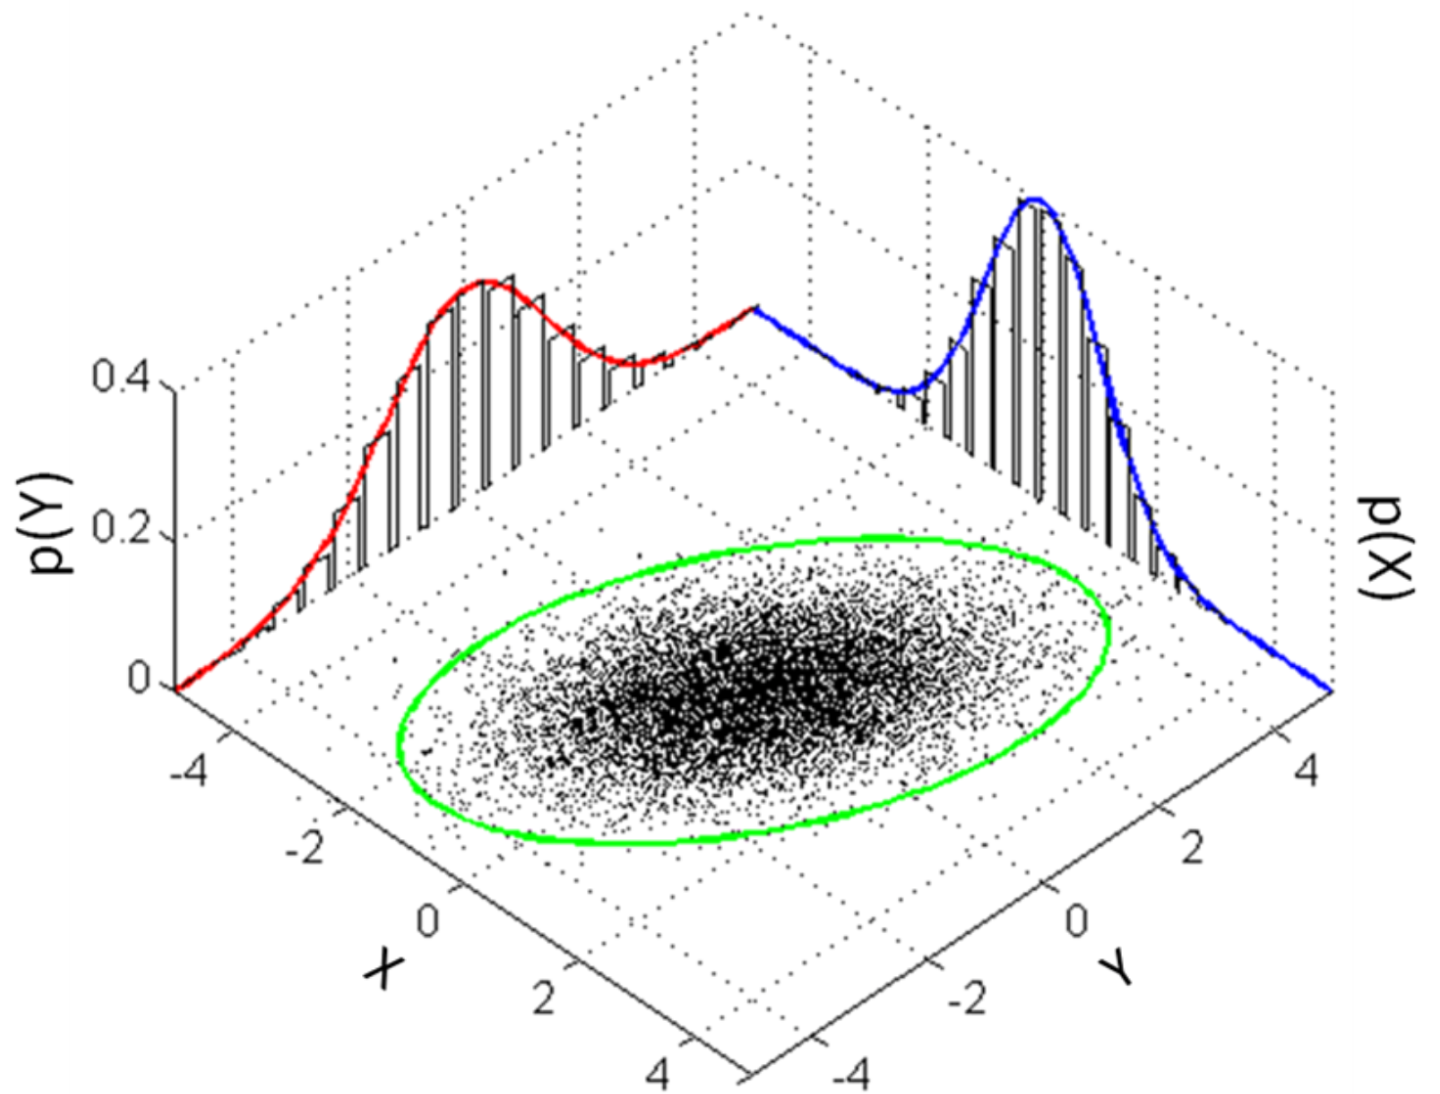
\includegraphics[width=3.25in]{stuff/joint.png} 

\textcolor{gray}{\emph{This multivariate normal joint distribution models the strength of relationship between $X$ and $Y$ with a correlation parameter $\rho$ and it's marginal distributions that are themselves normally distributed}}
\end{figure}
}


\frame
{
 \frametitle{Joint Distributions}%\frametitle{Marginal Distributions/ L of total P} % \frametitle{Bayes Theorem}

\begin{itemize}
\item \emph{Errata:} joint distribution \textbf{is allowed/encouraged} on campus\\${}$

\fbox{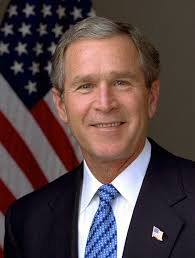
\includegraphics[height=.75in]{stuff/2016-12-06-16-18-09-39796758.jpg}
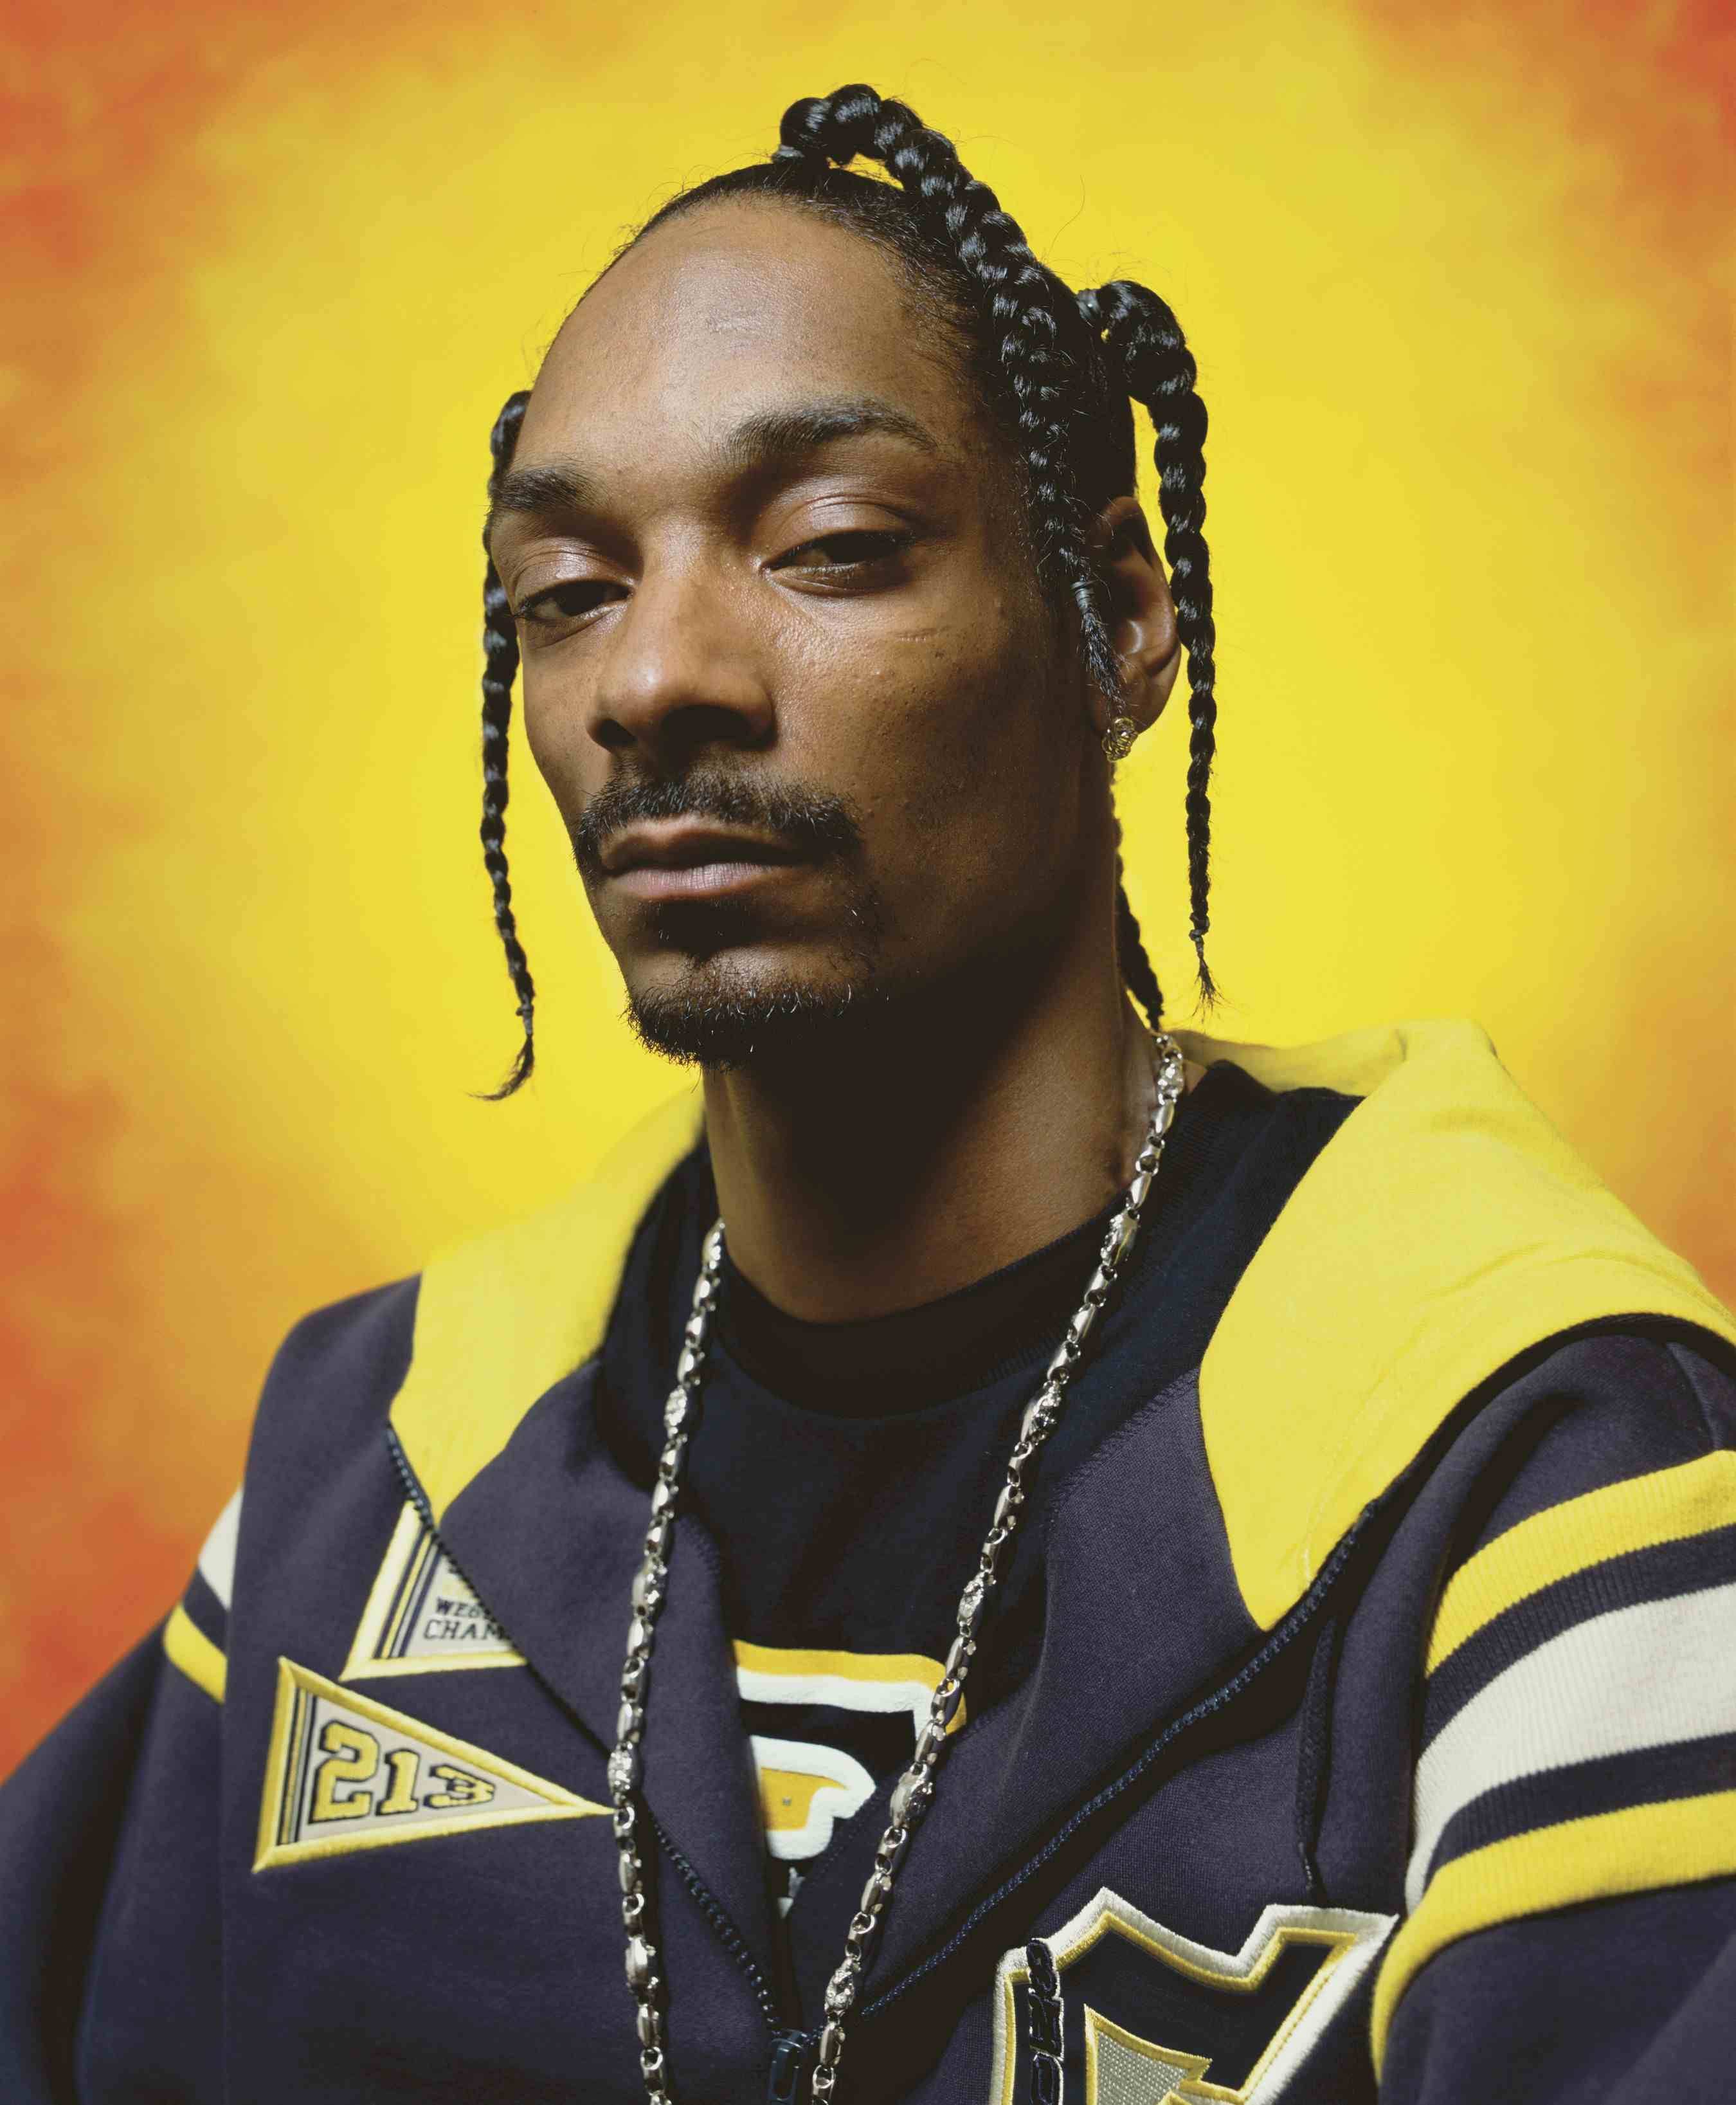
\includegraphics[height=.75in]{stuff/Snoop-Dogg-Hairstyle.jpg}
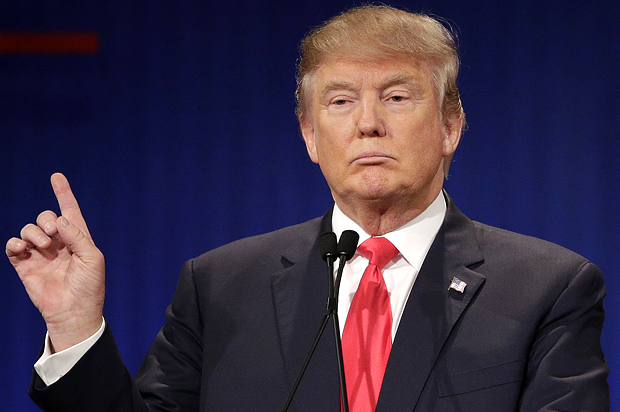
\includegraphics[height=.75in]{stuff/donald_trump69.jpg}

\includegraphics[height=.75in]{stuff/mmikes.png}%_400x300.png}
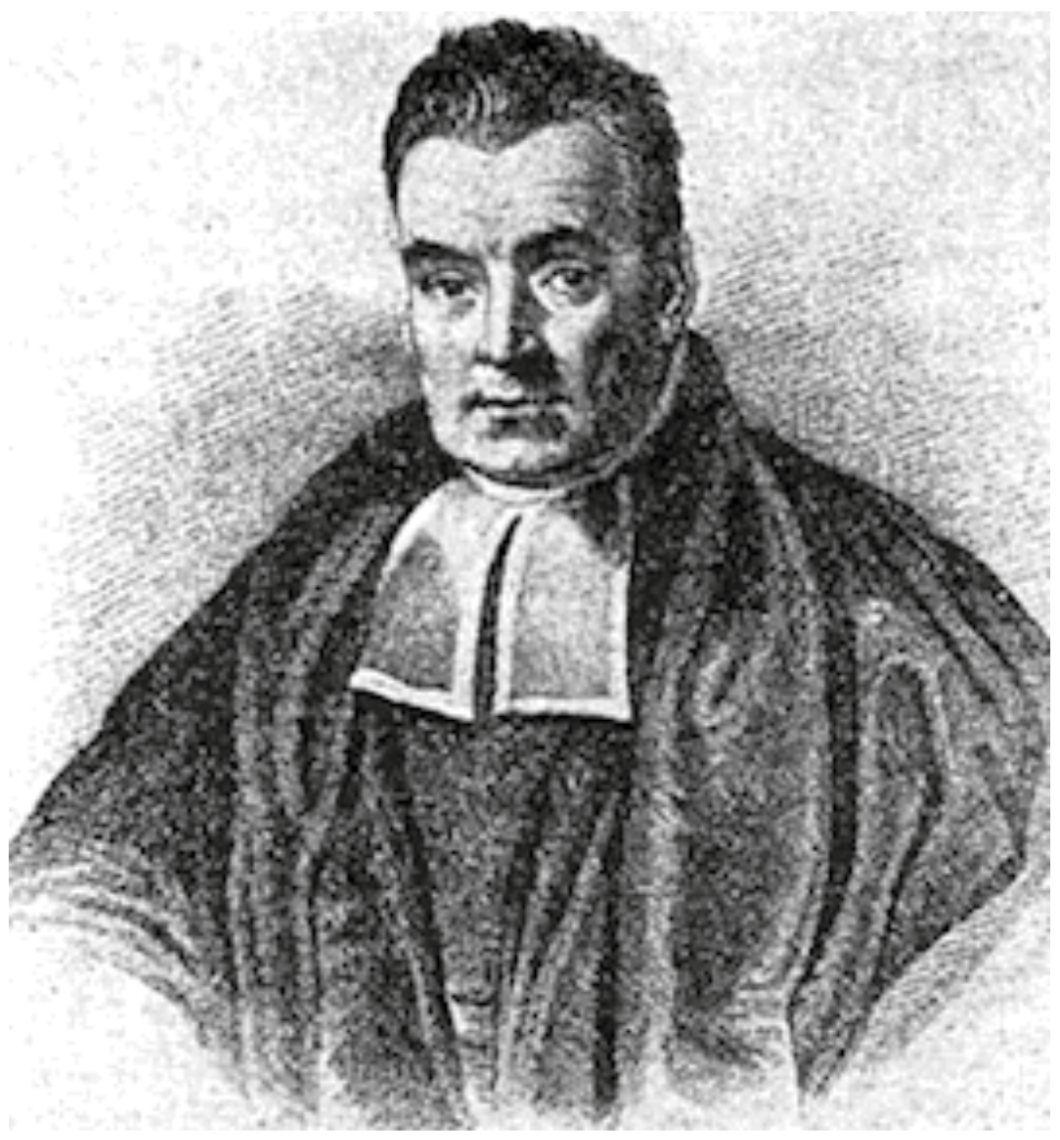
\includegraphics[height=.75in]{stuff/bayes.png}}\\${}$

\item<2->[] \emph{Joint distributions} are just a collection of random variables that may or may not
have some dependencies on each other
$$ \Pr(X_1,X_2,\cdots,X_k) $$

%\item Let $X_j$ be the number of joints Snoop Dogg's sells to client $j$ 
%\item<2-> We model Snoop's joint distribution with a \emph{joint distribution}
%\item<3-> We'll use a \emph{multinomial distribution} for the \emph{joint distribution} 
\item<3-> \textcolor{NavyBlue}{We actually already saw an example of a \emph{joint distribution}}
$$\textcolor{NavyBlue}{\Pr(\textbf{X}=\textbf{x}|\theta_1, \theta_2,\cdots \theta_k, m) = \frac{m!}{x_1!x_2!\cdots x_k!}  \prod_{j=1}^k \theta_j^{x_j} 
\text{}}$$

\hspace{.69in}\textcolor{gray}{Do these $X_j$'s have some \emph{dependence}?}

%\item<6-> (\emph{multinomial distribution})

\end{itemize}
}



\frame
{
 \frametitle{Joint Distributions: \emph{discrete}}%\frametitle{Marginal Distributions/ L of total P} % \frametitle{Bayes Theorem}

\begin{itemize}
\item \emph{Joint distributions} factor as \emph{conditional} $\times$ \emph{marginal} dist.'s
$$\Pr(\textbf{X}_1,\textbf{X}_2) =  \Pr(\textbf{X}_1|\textbf{X}_2) \Pr(\textbf{X}_2)$$
\item<2->  \emph{Bayes theorem} is derived from joint distribution factoring
$$\Pr(\textbf{X}_2|\textbf{X}_1) = \frac{\Pr(\textbf{X}_1|\textbf{X}_2)\Pr(\textbf{X}_2)}{\Pr(\textbf{X}_1)}$$
\item<3-> \emph{Independence} of $\textbf{X}_1$ and $\textbf{X}_2$ is when
$$\Pr(\textbf{X}_1|\textbf{X}_2) =  \Pr(\textbf{X}_1), \text{ or}\quad\;\;$$ 
$$\Pr(\textbf{X}_1,\textbf{X}_2) = \Pr(\textbf{X}_1)\Pr(\textbf{X}_2)$$

\item<4->  \emph{Marginal distributions} are derived from \emph{joint distributions}
$$\Pr(\textbf{X}_1) = \sum_{x_2 \in \mathcal{S}_{X_2}} \Pr(\textbf{X}_1,X_2=x_2) $$ 

\end{itemize}
}


\frame
{
 \frametitle{Joint Distributions: \emph{continuous}}%\frametitle{Marginal Distributions/ L of total P} % \frametitle{Bayes Theorem}

\begin{itemize}
\item \emph{Joint distributions} factor as \emph{conditional} $\times$ \emph{marginal} dist.'s
$$f(\textbf{X}_1,\textbf{X}_2) =  f(\textbf{X}_1|\textbf{X}_2) f(\textbf{X}_2)$$
\item  \emph{Bayes theorem} is derived from joint distribution factoring
$$f(\textbf{X}_2|\textbf{X}_1) = \frac{f(\textbf{X}_1|\textbf{X}_2)f(\textbf{X}_2)}{f(\textbf{X}_1)}$$
\item \emph{Independence} of $\textbf{X}_1$ and $\textbf{X}_2$ is when
$$f(\textbf{X}_1|\textbf{X}_2) =  f(\textbf{X}_1), \text{ or}\;\;\;$$ 
$$f(\textbf{X}_1,\textbf{X}_2) = f(\textbf{X}_1)f(\textbf{X}_2)$$

\item  \emph{Marginal distributions} are derived from \emph{joint distributions}
$$f(\textbf{X}_1) = \int_{ \mathcal{S}_{X_2}} f(\textbf{X}_1,X_2=x_2) dx_2 $$ 

\end{itemize}
}


\frame
{
 \frametitle{\emph{Expectation, Variance, Covariance and Correlation}}
%$\textrm{E}[aX], \textrm{Var}[X], \textrm{E}[XY+Z]$ and $\textrm{Var}[aX+bY]$

\vspace{.75em}

\LARGE
\textbf{For Discrete DISTRIBUTIONS}
\small

\begin{itemize}
\item \textcolor{gray}{The \emph{Expected Value} of $X$} $\displaystyle \text{E}_X[X] = \sum_{x \in \mathcal{S}_{X}} x\Pr(X=x)$

\vspace{.5em}
\item<2->  ${}$

\vspace{-3.5em}
\begin{align*}  
\text{\textcolor{gray}{The \emph{Variance} of $X$} Var}[X] = {} & \sum_{x \in \mathcal{S}_{X}} (x-\text{E}_X[X])^2 \Pr(X=x) \quad\quad \\
= {} & \text{E}_X[X^2] - \text{E}_X[X]^2 
\end{align*}

\vspace{-1em}
\item<3-> \textcolor{gray}{The \emph{Covariance} of $X$ \& $Y$} 
\item<3->[] $\displaystyle  \text{Cov}(X,Y) = \sum_{(x,y) \in \mathcal{S}_{XY}} (x-\text{E}_X[X])(y-\text{E}_Y[Y]) \Pr(X=x,Y=y)$

\item<4-> \textcolor{gray}{The \emph{Correlation} of $X$ \& $Y$ } $\text{Cor}(X,Y) = \frac{\text{Cov}(X,Y)}{\sqrt{\text{Var}[X]\text{Var}[Y] }}$ \footnotesize \textcolor{gray}{$\in [-1, 1]$} \normalsize
\item<5-> \textcolor{gray}{For $a, b, c \in \mathbb{R}, \;\; \text{E}[aX+bY+c] = \text{?}$}
\item<6-> \textcolor{gray}{$\text{Var}[aX+bY+ c] \overset{?}{=} a^2\text{Var}[X] + b^2\text{Var}[Y] + 2ab \text{Cov}(X,Y)$}   
\item<7-> \textcolor{gray}{If $X$ and $Y$ are \emph{independent},  $\text{E}_{XY}[XY] \overset{?}{=} \text{E}_X[X]\text{E}_Y[Y]$}
\end{itemize}

%distinguish between joint/univariate distribution concepts
}

\frame
{
 \frametitle{\emph{Expectation, Variance, Covariance and Correlation}}
%$\textrm{E}[aX], \textrm{Var}[X], \textrm{E}[XY+Z]$ and $\textrm{Var}[aX+bY]$

\vspace{.75em}
\LARGE
\textbf{For Continuous DISTRIBUTIONS}
\small

\begin{itemize}
\item \textcolor{gray}{The \emph{Expected Value} of $X$} $\displaystyle \text{E}_X[X] = \int_{x \in \mathcal{S}_{X}} x\; f(X=x) dx$

\vspace{.3em}
\vspace{.5em}
\item  ${}$

\vspace{-3.5em}
\begin{align*}  
\text{\textcolor{gray}{The \emph{Variance} of $X$} Var}[X] = {} & \int_{x \in \mathcal{S}_{X}} (x-\text{E}_X[X])^2 \; f(X=x)dx \quad\quad \\
= {} & \text{E}_X[X^2] - \text{E}_X[X]^2 
\end{align*}

\vspace{.3em}

\vspace{-1em}
\item \textcolor{gray}{\emph{The Covariance} of $X$ and $Y$} 
\item[] $ \text{Cov}(X,Y) = \displaystyle \int_{\overset{(x,y)}{\in \mathcal{S}_{XY}}} (x-\text{E}_X[X])(y-\text{E}_Y[Y]) f(X=x,Y=y)d_{xy}$
\item \textcolor{gray}{The \emph{Correlation} of $X$ \& $Y$ } $\text{Cor}(X,Y) = \frac{\text{Cov}(X,Y)}{\sqrt{\text{Var}[X]\text{Var}[Y] }}$ \footnotesize \textcolor{gray}{$\in [-1, 1]$} \normalsize

\item \textcolor{gray}{For $a, b, c \in \mathbb{R}, \;\; \text{E}[aX+bY+c] = \text{?}$}
\item \textcolor{gray}{$\text{Var}[aX+bY+ c] \overset{?}{=} a^2\text{Var}[X] + b^2\text{Var}[Y] + 2ab \text{Cov}(X,Y)$}   
\item \textcolor{gray}{If $X$ and $Y$ are \emph{independent},  $\text{E}_{XY}[XY] \overset{?}{=} \text{E}_X[X]\text{E}_Y[Y]$}
\end{itemize}

%distinguish between joint/univariate distribution concepts
}


\frame
{
 \frametitle{\emph{Expectation, Variance, Covariance and Correlation}}
%$\textrm{E}[aX], \textrm{Var}[X], \textrm{E}[XY+Z]$ and $\textrm{Var}[aX+bY]$

\LARGE
\textbf{For SAMPLES we have \emph{STATISTICS}}\\

\vspace{.5em}
\Large
\textcolor{NavyBlue}{Statistics are functions of the original random variables \emph{and hence are themselves random variables}}
\normalsize

\vspace{1.75em}
\begin{itemize}
\item<2-> \textcolor{gray}{The \emph{Sample Mean} } $\displaystyle \bar X = \frac{1}{n}\sum_{i=1}^n X_i$

\item<3->  \textcolor{gray}{The \emph{Sample Variance}}  $\displaystyle S^2_X = \frac{1}{n-1}\sum_{i=1}^n (X_i-\bar X)^2$

\item<4-> \textcolor{gray}{The \emph{Sample Covariance}}  $\displaystyle S_{XY} = \frac{1}{n-1}\sum_{i=1}^n (X_i-\bar X)(Y_i-\bar Y)$

\item<5-> \textcolor{gray}{The \emph{Sample Correlation$^*$}}  $\displaystyle R_{XY} = \frac{S_{XY}}{\sqrt{S_{X}^2S_{Y}^2 }}$  \textcolor{gray}{$\in [-1, 1]$} \\
\scriptsize
\textcolor{gray}{$^*$not robust... correlation of ranks?}
\end{itemize}
}


\frame
{
 \frametitle{\emph{Why $n-1$?}}

\tiny 
\begin{align*} 
E\left[\sum_{i=1}^n\left(x_i^2-\frac{1}{n}\sum_{j=1}^nx_j\right)^2\right] 
= {}& E\left[\sum_{i=1}^n\left(x_i^2-\frac{2x_i}{n}\sum_{j=1}^nx_j + 
\left(\frac{1}{n}\sum_{j=1}^nx_j\right)^2\right)\right] \\ 
= {}& E\left[\sum_{i=1}^nx_i^2-\textcolor{blue}{\frac{2}{n} \sum_{i=1}^n \sum_{j=1}^nx_ix_j} + 
\textcolor{red}{\frac{1}{n} \sum_{i=1}^n\sum_{j=1}^nx_ix_j}\right] \\ 
= {}& E\left[\sum_{i=1}^nx_i^2 - \textcolor{blue}{\frac{2}{n}\sum_{i=1}^nx_i^2 -\frac{2}{n}\sum_{j\not=i}x_ix_j} + 
\textcolor{red}{\frac{1}{n}\sum_{i=1}^nx_i^2 + \frac{1}{n}\sum_{j\not=i}x_ix_j} \right] \\
= {}& E\left[\sum_{i=1}^nx_i^2 - \textcolor{blue}{\frac{2}{n}\sum_{i=1}^nx_i^2} + \textcolor{red}{\frac{1}{n}\sum_{i=1}^nx_i^2} 
 -\textcolor{blue}{\frac{2}{n}\sum_{j\not=i}x_ix_j}  
 + \textcolor{red}{\frac{1}{n}\sum_{j\not=i}x_ix_j} \right] \\
 = {}& E\left[\textcolor{black}{\frac{n-1}{n}\sum_{i=1}^nx_i^2} 
 -\textcolor{black}{\frac{1}{n}\sum_{j\not=i}x_ix_j}  \right] = \textcolor{black}{\frac{n-1}{n}\sum_{i=1}^n E\left[x_i^2\right] } 
 -\textcolor{black}{\frac{1}{n} \sum_{j\not=i} E\left[x_ix_j\right] }   \\ 
 = {}& \textcolor{black}{\frac{n-1}{n}\sum_{i=1}^n (\sigma^2 + \mu^2) } 
 -\textcolor{black}{\frac{1}{n} \sum_{j\not=i} \mu^2 } \quad (\text{\emph{why?}})  \\ 
 = {}& \textcolor{black}{(n-1) (\sigma^2 + \mu^2) } 
 -\textcolor{black}{\frac{n^2-n}{n} \mu^2 }   =  \textcolor{violet}{(n-1)\sigma^2}
\end{align*}

}

\frame
{
 \frametitle{Bias versus Variance of Estimators}

\hspace{3em}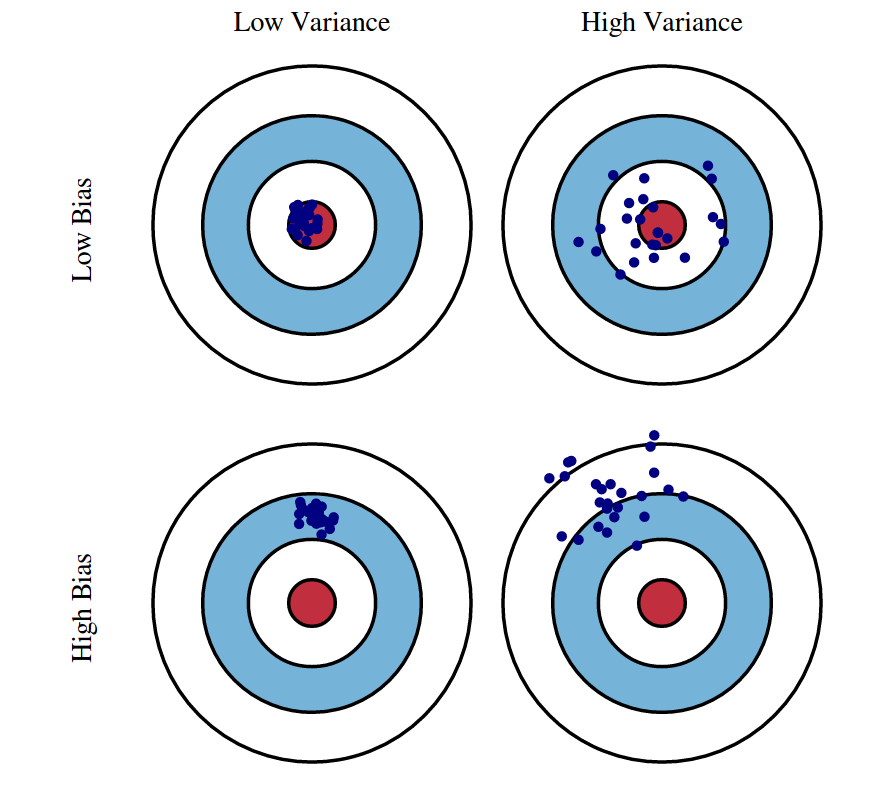
\includegraphics[width=3in]{stuff/bullseye.png}
}

 

\frame
{
 \frametitle{\emph{Covariance is not Correlation is not Causation}}

$$\text{Cov}[X,Y] \not = \text{Cor}[X,Y] \; \textcolor{gray}{= \frac{\text{Cov}[X,Y]}{\sqrt{\text{Var}[X]\text{Var}[Y] }}}$$



\begin{figure}[h!]
   \centering
   
and ``correlation \emph{is not} causation''\\
\textcolor{gray}{or more generally, ``association \emph{is not} causation''}\\${}$

\onslide<2->{Conversely, \emph{uncorrelated variables} \textbf{are not} necessarily \emph{independent}\\
   
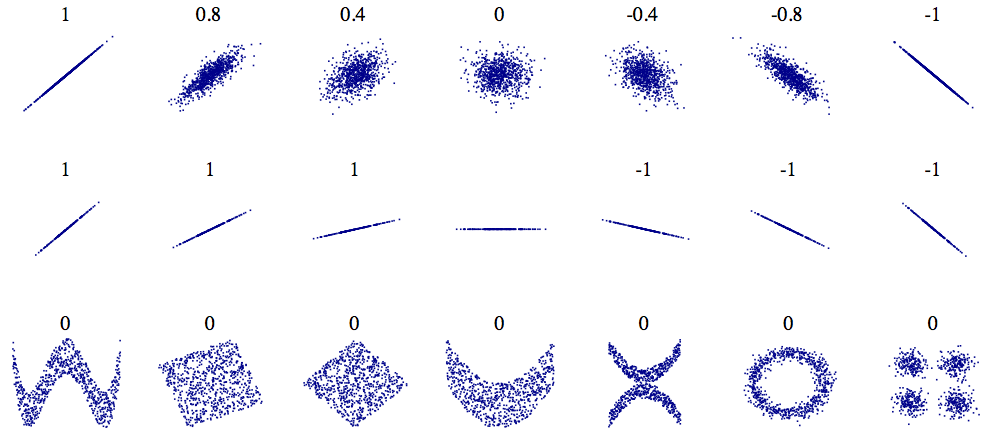
\includegraphics[width=3.5in]{stuff/cors.png}  \\${}$\\}

\scriptsize
\onslide<3->{\textcolor{Maroon}{$^*$\underline{Mutually exclusive} events $E_1$ and $E_2$ \underline{quite dependent} }\textcolor{NavyBlue}{(as opposed to independent)}}
\end{figure}  


%$\textrm{E}[aX], \textrm{Var}[X], \textrm{E}[XY+Z]$ and $\textrm{Var}[aX+bY]$

% emphasize distinction between these and independence and mutually exclusive
}





\end{document}


\begin{columns}
\begin{column}{.66\textwidth}
\includegraphics[width=1in]{snoop-dogg.jpg}

\includegraphics[width=1in]{16_3billionjoints.jpg}

\end{column}
\begin{column}{.33\textwidth}
\includegraphics[height=.3in]{adamsandburg.jpg}
 
\includegraphics[height=.3in]{_Tyrone20Biggums.jpg}

\includegraphics[height=.3in]{georgebush.jpg}
\end{column}
\end{columns}
}



\frame
{
 \frametitle{Beating the House}

\tiny
\begin{columns}
\begin{column}{.3\textwidth}
\begin{tabular}{|l|l|}
\hline
& House \\
Game & Advantage \\  \hline
Baccarat (no tie bets) &1.2\% \\ \hline
Craps (pass/come) &  1.4\% \\ \hline
Blackjack (average player) & 2.0\% \\ \hline
Video Poker (average player) & 0.5\% - 3\% \\ \hline
Roulette (double-zero) & 5.3\% \\ \hline
Slots & 5.0\%-10.0\% \\ \hline
Keno (average) & 27.0\% \\\hline 
\end{tabular}
\end{column}
\begin{column}{.375\textwidth}
\vspace{1em}
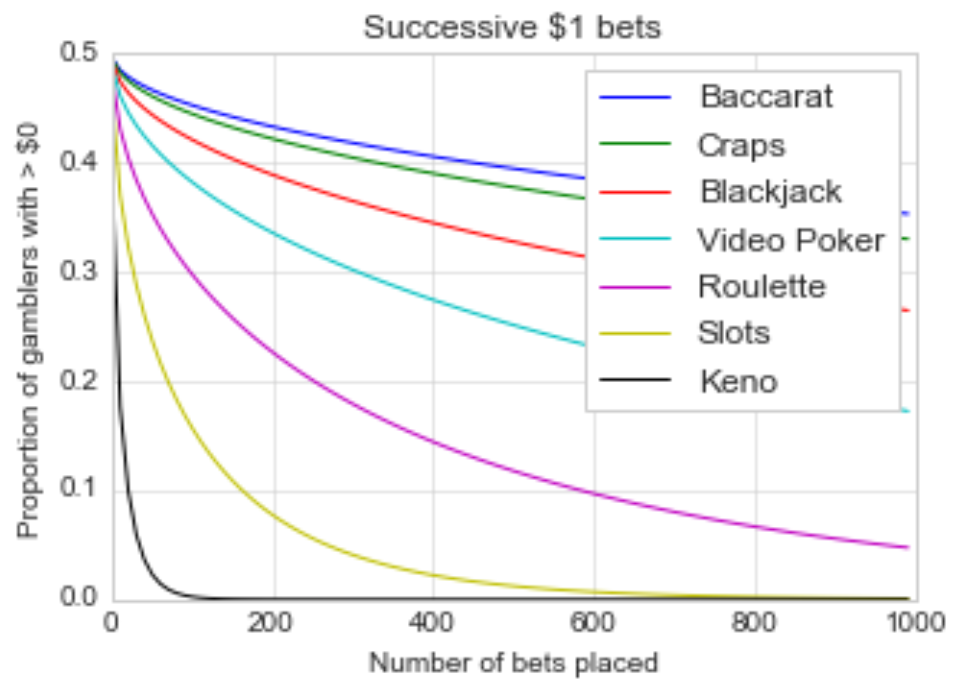
\includegraphics[width=1.65in]{vegas.png}  
\end{column}
\end{columns}

{
\fontfamily{<familyname>}\selectfont
\begin{quote}
\tiny
\justify


Blackjack can be legally beaten by keeping track of the probability of getting a high card (10,J,Q,K,A) compared to a low card (2,3,4,5,6). This is called $card$ $counting$.  
In early 1979, four MIT students taught themselves card counting and along with a professional gambler and an investor who put up most of their capital (\$5,000) went to Atlantic City for spring break.  They went again in December and then recruited a few more MIT students as ``students'' for a ``blackjack class''. The ``class'' continued to visit Atlantic City intermittently until May 1980 (when the students graduated), during which time they increased their capital four-fold.  
At about the same time, Bill Kaplan returned to Cambridge after successfully running a blackjack team in Las Vegas.  Kaplan earned his BA at Harvard in 1977 and was accepted into Harvard Business School but delayed admission while he ran the blackjack team. Kaplan ran his operation using funds he received upon graduation as Harvard's ``outstanding scholar-athlete'' and generated more than a 35 fold rate of return in less than nine months of play.  Kaplan continued to run his Las Vegas blackjack team as a sideline while attending Harvard Business School but by the time of his graduation the players were so ``burnt out" the team disbanded. 
\end{quote}
}
}




\frame
{

\xymatrix{
&&&& 0.000199 \\
& \text{Test?} \ar[urrr]^{\Pr(+|{Pox})}_{0.995} \ar[drrr]^{0.005}_{\Pr(\cancel{+}|{Pox})} &\\
&&& &  0.000001 \\
\text{Pox?} \ar[ddr]_{\Pr({\cancel{Pox}})}^{0.9998} \ar[uur]^{\Pr({Pox})}_{0.0002}&\\
 &&& & 0.09998 \\
& \text{Test?} \ar[urrr]^{\Pr(+|{\cancel{Pox}})}_{0.1}  \ar[drrr]^{0.9}_{\Pr(\cancel{+}|{\cancel{Pox}})}&\\
&&&& 0.89982 \\
}
}


\frame
{

\xymatrix{
&&&&  0.99 \times 0.5^{10} \\
& \text{10/10 heads?} \ar[urrr]^{\Pr(10/10|{Fair})}_{0.5^{10}} \ar[drrr]^{1-0.5^{10}}_{\Pr(\cancel{10/10}|{Fair})} &\\
&&& & 0.99 \times (1-0.5^{10})  \\
\text{Fair?} \ar[ddr]_{\Pr({\cancel{Fair}})}^{0.01} \ar[uur]^{\Pr({Fair})}_{0.011}&\\
 &&& & 0.01 \\
& \text{10/10 heads?} \ar[urrr]^{\Pr(10/10|{\cancel{Fair}})}_{1}  \ar[drrr]^{0}_{\Pr(\cancel{10/10 }|{\cancel{Fair}})}&\\
&&&& 0 \\
}
}


\frame
{
 \frametitle{Problem 3:}

\begin{columns}
\begin{column}{.55\textwidth}

\vspace{-1.5em}

\begin{itemize}
\item[]
\footnotesize
\begin{align*}
\Pr(Trump_{Fantastic}) = & 0.20\\
Pr(DS_{Job} | Trump_{Fantastic}) = {} & 0.98\\
Pr(DS_{Job} | Trump_{\cancel{Fantastic}}) = {} & 0.90\\{}\\
Pr(Trump_{Fantastic} | DS_{Job} ) = {} & ?
\end{align*}

\item[]<3->
\vspace{-1em}
\footnotesize
\begin{align*}
\Pr(DS_{Job} \& Trump_{Fantastic}) = {} & 0.20 \cdot 0.98\\
\Pr(DS_{\cancel{Job}} \& Trump_{Fantastic}) = {} & 0.20 \cdot 0.02\\
\Pr(DS_{{Job}} \& Trump_{\cancel{Fantastic}}) = {} & 0.80 \cdot 0.90\\
\Pr(DS_{\cancel{Job}} \& Trump_{\cancel{Fantastic}}) = {} & 0.80 \cdot 0.10\\
\end{align*}

\item[]<4->
\vspace{-1em}
\begin{tabular}{m{1.1cm}|m{1.5cm}m{1.5cm}|m{1.5cm}}  %{c|cc|c}
                           & $\underset{Fantastic}{Trump}$ & $\underset{\cancel{Fantastic}}{Trump}$ & $\underset{\text{Marginal prob}}{DS}$\\ \hline
$\quad\;\;\underset{Job}{DS}$ &  $\;\;\;$\textcolor{red}{0.196} & $\;\;\;$\textcolor{red}{0.720} & $\;\;\;$\textcolor{red}{0.916} \\
$\quad\;\;\underset{\cancel{Job}}{DS}$ & $\;\;\;$0.004 & $\;\;\;$0.080 & $\;\;\;$0.084 \\\hline
 $\underset{\text{Marginal prob}}{Trump}$& $\;\;\;$0.200 & $\;\;\;$0.800 & $\;\;\;$1.000
\end{tabular}

\end{itemize}
\end{column}
\begin{column}{.45\textwidth}

\begin{itemize}
\item[]<2->
\vspace{-2em}
\tiny
\xymatrix{
&& 0.196 \\
& \text{Election} \ar[ur]^{\Pr(Job{Fantastic})}_{0.98} \ar[dr]^{0.02}_{\Pr(\cancel{Job}|{Fantastic})} &\\
& &  0.004 \\
\text{Hillary} \ar[ddr]_{\Pr({\cancel{Fantastic}})}^{0.8} \ar[uur]^{\Pr({Fantastic})}_{0.2}&\\
 & & 0.72 \\
& \text{Election} \ar[ur]^{\Pr(Job|{\cancel{Fantastic}})}_{0.9}  \ar[dr]^{0.1}_{\Pr(\cancel{Job}|{\cancel{Fantastic}})}&\\
&& 0.08 \\
}
\item[]<5->
\large
\vspace{-1em}
$$\color{red}{\frac{0.196}{0.916}}$$

\end{itemize}
\end{column}
\end{columns}

\begin{itemize}
\item[]<4->
$$\Pr( Trump_{Fantastic} | DS_{Job} ) = \frac{\Pr( Trump_{Fantastic} \& DS_{Job}) }{\Pr(DS_{Job})}$$
\end{itemize}

%U \ar@/_/[ddr]_y \ar@/^/[drr]^x
 %  \ar@{.>}[dr]|-{(x,y)}            \\
 % & X \times_Z Y \ar[d]^q \ar[r]_p
 %                & X \ar[d]_f       \\
 % & Y \ar[r]^g   & Z                

}


\end{document}


